\documentclass[conference]{IEEEtran}

\usepackage[utf8]{inputenc}
\usepackage[T1]{fontenc}
\usepackage[spanish,es-nodecimaldot,es-noquoting]{babel}
\usepackage{amsmath,amssymb}
\usepackage{graphicx}
\usepackage{booktabs}
\usepackage{array}
\usepackage{cite}
\usepackage{url}
\usepackage[american]{circuitikz}
\usetikzlibrary{babel}

\graphicspath{{./}{./Figuras/}}

\renewcommand{\tablename}{Tabla}
\renewcommand{\figurename}{Fig.}

\begin{document}

\title{Caracterizaci\'on del Transistor BJT 2N3904 y Dise\~no de Amplificadores de Peque\~na Se\~nal en Configuraciones B\'asicas y en Cascada}

\author{
\IEEEauthorblockN{Nombre Estudiante 1}
\IEEEauthorblockA{Ingenier\'ia Electr\'onica\\
Universidad Nacional de Colombia\\
Bogot\'a, Colombia\\
correo1@unal.edu.co}
\and
\IEEEauthorblockN{Nombre Estudiante 2}
\IEEEauthorblockA{Ingenier\'ia Electr\'onica\\
Universidad Nacional de Colombia\\
Bogot\'a, Colombia\\
correo2@unal.edu.co}
\and
\IEEEauthorblockN{Nombre Estudiante 3}
\IEEEauthorblockA{Ingenier\'ia Electr\'onica\\
Universidad Nacional de Colombia\\
Bogot\'a, Colombia\\
correo3@unal.edu.co}
}

\maketitle

\begin{abstract}
En este documento se presenta el trabajo previo de dise\~no, an\'alisis anal\'itico y validaci\'on por simulaci\'on en LTspice correspondiente a la Pr\'actica 5 de Electr\'onica An\'aloga I sobre el transistor de uni\'on bipolar (BJT) 2N3904. Se caracteriza inicialmente la ganancia de corriente directa $\beta$ y las regiones de operaci\'on del dispositivo, integrando resultados simulados y experimentales previos ($\beta_{\mathrm{prom1}} = 212.58$ y $\beta_{\mathrm{prom2}} = 246.13$). Posteriormente, se dise\~nan y eval\'uan las configuraciones de emisor com\'un degenerado, colector com\'un y amplificador en cascada (emisor com\'un seguido de colector com\'un) con $V_{CC} = 12\text{ V}$ y $R_L = 10\text{ k}\Omega$, reservando el espacio indicado para la etapa individual de emisor com\'un. La etapa en cascada alcanza una ganancia simulada en banda media de $152.78\text{ V/V}$ ($43.68\text{ dB}$), impedancia de entrada de $2.37\text{ k}\Omega$ y ancho de banda de $9.52\text{ MHz}$, con errores relativos inferiores al $2.3\%$ respecto al modelo anal\'itico.
\end{abstract}

\begin{IEEEkeywords}
Amplificador en cascada, BJT 2N3904, colector com\'un, emisor degenerado, peque\~na se\~nal, polarizaci\'on DC.
\end{IEEEkeywords}

\section{Introducci\'on y justificaci\'on}

El transistor de uni\'on bipolar (BJT, por sus siglas en ingl\'es) constituye uno de los dispositivos activos fundamentales en el procesamiento anal\'ogico de se\~nales. Su principio de operaci\'on se basa en el control de una corriente de colector $I_C$ mediante una corriente de base $I_B$ o el voltaje base-emisor $V_{BE}$, exhibiendo tres regiones principales de funcionamiento: corte, saturaci\'on y regi\'on activa directa \cite{sedra2020}. Para aplicaciones de amplificaci\'on lineal de peque\~na se\~nal, el transistor debe polarizarse firmemente en la regi\'on activa directa, donde la uni\'on base-emisor est\'a polarizada en directa y la uni\'on base-colector en inversa, permitiendo modelar su comportamiento incremental mediante la red h\'ibrida-$\pi$ y los par\'ametros de transconductancia $g_m$, resistencia de entrada $r_\pi$ y resistencia de salida por efecto Early $r_o$ \cite{sedra2020}.

El objetivo general de esta pr\'actica es aplicar la teor\'ia de polarizaci\'on y an\'alisis de peque\~na se\~nal en BJT para dise\~nar y validar amplificadores en configuraciones de emisor com\'un (EC), emisor com\'un degenerado (ECD), colector com\'un (CC) y su interconexi\'on en cascada (EC--CC), evaluando la ganancia de tensi\'on $A_v$, las impedancias $Z_{\mathrm{in}}$ y $Z_{\mathrm{out}}$, los l\'imites de peque\~na se\~nal y la respuesta en frecuencia con el transistor 2N3904 \cite{onsemi2021}.

El dominio de estas topolog\'ias discretas posee alta relevancia en m\'ultiples sectores tecnol\'ogicos. En la industria m\'edica, las etapas de entrada de bajo ruido y acoplamiento de impedancias basadas en transistores bipolares resultan esenciales para acondicionar biopotenciales de amplitud microvolt\'aica, como se\~nales electrocardiogr\'aficas y electroencefalogr\'aficas, sin cargar los electrodos ni degradar la relaci\'on se\~nal a ruido \cite{webster2010}. En el sector de telecomunicaciones, las configuraciones EC, degeneradas y seguidores de emisor se emplean extensamente en amplificadores de bajo ruido, etapas de frecuencia intermedia y acopladores de banda ancha gracias a la elevada transconductancia por unidad de corriente del BJT \cite{razavi2012}. Asimismo, en sistemas aeroespaciales y de telemetr\'ia satelital, el dise\~no de etapas anal\'ogicas bipolares estables frente a variaciones t\'ermicas y tolerancias de par\'ametros garantiza la confiabilidad en la adquisici\'on de sensores de a bordo bajo condiciones ambientales extremas \cite{fortescue2011}. Complementariamente, el conocimiento de estas etapas b\'asicas constituye el bloque constructivo de circuitos integrados anal\'ogicos y sistemas de instrumentaci\'on de precisi\'on \cite{horowitz2015}.

\section{C\'alculos}

Para el desarrollo anal\'itico se emplea el modelo del transistor NPN 2N3904 \cite{onsemi2021}, considerando $V_{BE,\mathrm{on}} = 0.7\text{ V}$, $V_{CE,\mathrm{sat}} = 0.2\text{ V}$, voltaje t\'ermico $V_T = 25.85\text{ mV}$ a $300\text{ K}$ y tensi\'on de Early nominal $V_A = 100\text{ V}$ \cite{sedra2020}. Para la etapa de caracterizaci\'on se toma $\beta_{\mathrm{teo}} = 200$ (valor t\'ipico de hoja de datos para $h_{FE}$ entre $100$ y $300$ \cite{onsemi2021}), mientras que para el dise\~no de los amplificadores se incorpora la ganancia caracterizada del primer transistor f\'isico, $\beta = 212.58$, coherente con el modelo empleado en simulaci\'on.

\subsection{Caracterizaci\'on del transistor BJT 2N3904}

En el circuito de caracterizaci\'on mostrado en la Fig. \ref{fig:caract_esq}, la base se alimenta con $V_1 = 3\text{ V}$ a trav\'es de $R_2 = R$ y el colector con $V_2 = 10\text{ V}$ a trav\'es de $R_1 = 100\ \Omega$. Asumiendo la uni\'on base-emisor en conducci\'on directa, la corriente de base est\'a determinada por la ley de voltajes de Kirchhoff en la malla de entrada:
\begin{equation}
I_B = \frac{V_1 - V_{BE,\mathrm{on}}}{R}
\label{eq:ib_caract}
\end{equation}
La ecuaci\'on \eqref{eq:ib_caract} evidencia que $I_B$ decrece de manera inversamente proporcional al incremento logar\'itmico de $R$.

\begin{figure}[htbp]
\centering
\resizebox{0.82\linewidth}{!}{%
\begin{circuitikz}
\draw (3.6, 1.5) node[npn](Q1){};
\node[right=4pt] at (Q1.C |- Q1.B) {\shortstack[l]{$Q_1$\\2N3904}};
\draw (Q1.E) -- (Q1.E |- 0,0) node[ground]{};
\draw (0,0) to[battery1, l={$V_1$}, a={$3\ \mathrm{V}$}] (0,0 |- Q1.B)
      to[R, l={$R_2$}, a={$R$}] (Q1.B);
\draw (0,0) to[short, -*] (Q1.E |- 0,0);
\draw (Q1.C) to[short, *-o] ++(0.9,0) node[right]{$V_C$};
\draw (Q1.C) to[R, l={$R_1$}, a={$100\ \Omega$}] ++(0,2.2) coordinate (topC);
\draw (topC) -- (6.2,0 |- topC) coordinate (topV2);
\draw (6.2,0) to[battery1, l={$10\ \mathrm{V}$}, a={$V_2$}] (topV2);
\draw (Q1.E |- 0,0) -- (6.2,0);
\end{circuitikz}%
}
\caption{Esquem\'atico del circuito de caracterizaci\'on del transistor BJT 2N3904 ($R$ barrida de $10\ \Omega$ a $100\text{ k}\Omega$).}
\label{fig:caract_esq}
\end{figure}

Si el dispositivo opera en saturaci\'on, la corriente m\'axima de colector queda acotada por la malla de salida mediante:
\begin{equation}
I_{C,\mathrm{sat}} = \frac{V_2 - V_{CE,\mathrm{sat}}}{R_1}
\label{eq:icsat}
\end{equation}
Evaluando \eqref{eq:icsat} con $V_2 = 10\text{ V}$, $V_{CE,\mathrm{sat}} = 0.2\text{ V}$ y $R_1 = 100\ \Omega$ se obtiene $I_{C,\mathrm{sat}} = 98.0\text{ mA}$.

El l\'imite te\'orico entre saturaci\'on y regi\'on activa ocurre cuando $I_B = I_{C,\mathrm{sat}}/\beta_{\mathrm{teo}}$, lo que define la resistencia cr\'itica de frontera:
\begin{equation}
R_{\mathrm{frontera}} = \frac{\beta_{\mathrm{teo}}(V_1 - V_{BE,\mathrm{on}})}{I_{C,\mathrm{sat}}}
\label{eq:rfront}
\end{equation}
Al sustituir los par\'ametros nominales en \eqref{eq:rfront} resulta $R_{\mathrm{frontera}} = 4.69\text{ k}\Omega$. Para $R > R_{\mathrm{frontera}}$, el transistor ingresa en regi\'on activa directa y sus variables de salida se calculan mediante:
\begin{equation}
I_C = \beta_{\mathrm{teo}} I_B, \qquad V_{CE} = V_2 - I_C R_1
\label{eq:activa_caract}
\end{equation}
La ecuaci\'on \eqref{eq:activa_caract} muestra que a medida que $R$ aumenta en la regi\'on activa, $I_C$ disminuye proporcionalmente y $V_{CE}$ tiende hacia $V_2 = 10\text{ V}$. La Tabla \ref{tab:caract_teo} resume los valores te\'oricos para el barrido por d\'ecadas entre $10\ \Omega$ y $100\text{ k}\Omega$.

\begin{table}[htbp]
\centering
\caption{Estimaci\'on te\'orica de la caracterizaci\'on del BJT 2N3904 ($\beta_{\mathrm{teo}} = 200$, $V_{BE} = 0.7\text{ V}$).}
\label{tab:caract_teo}
\begin{tabular}{@{}ccccc@{}}
\toprule
$R$ ($\Omega$) & $I_B$ (mA) & $I_C$ (mA) & $V_{CE}$ (V) & Regi\'on \\
\midrule
$10$ & $230.000$ & $98.00$ & $0.20$ & Saturaci\'on \\
$100$ & $23.000$ & $98.00$ & $0.20$ & Saturaci\'on \\
$1\,000$ & $2.300$ & $98.00$ & $0.20$ & Saturaci\'on \\
$10\,000$ & $0.230$ & $46.00$ & $5.40$ & Activa \\
$100\,000$ & $0.023$ & $4.60$ & $9.54$ & Activa \\
\bottomrule
\end{tabular}
\end{table}

% =========================================================================
% COMPAÑERO (EMISOR COMÚN): DESCOMENTAR Y COMPLETAR ESTA SUBSECCIÓN CON LOS
% CÁLCULOS ANALÍTICOS Y EL ESQUEMÁTICO EN CIRCUITIKZ DEL EMISOR COMÚN.
% =========================================================================
% \subsection{Amplificador en configuraci\'on emisor com\'un}
% % Insertar aquí el diseño de RB1, RB2, RC, RE, C1, C2, C3 para |Av| ≈ 5 V/V
% % con RL = 10 kOhm y señal de entrada de 50 mVpp a 10 kHz, junto con:
% % 1) Análisis DC (VTH, RTH, IB, IC, VCE).
% % 2) Análisis AC (gm, rpi, Av, Zin, Zout).
% % 3) Límites de pequeña señal y excursión máxima.
% % \begin{figure}[htbp]
% % \centering
% % \resizebox{0.86\linewidth}{!}{%
% % \begin{circuitikz}
% % \draw (4.5, 2.7) node[npn](Q1){};
% % \node[right=3pt] at (Q1.C |- Q1.B) {\shortstack[l]{$Q_1$\\2N3904}};
% % \draw (2.4, 5.6) to[R, l={$R_{B1}$}, a={$\mathrm{XX\ k}\Omega$}, -*] (2.4,0 |- Q1.B) coordinate (Bnode);
% % \draw (Bnode) to[R, l={$R_{B2}$}, a={$\mathrm{XX\ k}\Omega$}] (2.4, 0) node[ground]{};
% % \draw (Bnode) -- (Q1.B);
% % \draw (0,0 |- Bnode) node[left]{$V_{\mathrm{in}}$} to[C, o-, l={$C_1$}, a={$10\ \mu\mathrm{F}$}] (Bnode);
% % \draw (Q1.C |- 0, 5.6) to[R, l={$R_C$}, a={$\mathrm{XX\ k}\Omega$}] (Q1.C);
% % \draw (2.4, 5.6) to[short, -*] (3.5, 5.6) node[vcc]{$V_{CC}=12\ \mathrm{V}$} -- (Q1.C |- 0, 5.6);
% % \draw (Q1.E) to[R, l={$R_E$}, a={$\mathrm{XX}\ \Omega$}] (Q1.E |- 0, 0) node[ground]{};
% % \draw (Q1.E) to[short, *-] (6.1,0 |- Q1.E) to[C, l={$C_3$}, a={$10\ \mu\mathrm{F}$}] (6.1,0) node[ground]{};
% % \draw (Q1.C) to[C, *-, l={$C_2$}, a={$10\ \mu\mathrm{F}$}] (7.4,0 |- Q1.C) coordinate (OutNode);
% % \draw (OutNode) to[short, *-o] (8.0,0 |- OutNode) node[right]{$V_{\mathrm{out}}$};
% % \draw (OutNode) to[R, l={$R_L$}, a={$10\ \mathrm{k}\Omega$}] (OutNode |- 0, 0) node[ground]{};
% % \end{circuitikz}%
% % }
% % \caption{Esquem\'atico del amplificador en configuraci\'on emisor com\'un.}
% % \label{fig:ec_esq}
% % \end{figure}

\subsection{Amplificador en configuraci\'on emisor com\'un degenerado}

El dise\~no del amplificador en emisor com\'un degenerado, cuyo esquem\'atico se ilustra en la Fig. \ref{fig:ecd_esq}, emplea $V_{CC} = 12\text{ V}$, $R_{B1} = 47\text{ k}\Omega$, $R_{B2} = 6.8\text{ k}\Omega$, $R_C = 3.3\text{ k}\Omega$, $R_E = 470\ \Omega$, $R_L = 10\text{ k}\Omega$ y capacitores $C_1 = C_2 = 10\ \mu\text{F}$ para cumplir $|A_v| \approx 5\text{ V/V}$ manteniendo $Q_1$ en regi\'on activa. Mediante el equivalente de Th\'evenin en la base se obtienen $V_{TH}$ y $R_{TH}$:
\begin{equation}
V_{TH} = V_{CC}\frac{R_{B2}}{R_{B1}+R_{B2}}, \qquad R_{TH} = R_{B1} \parallel R_{B2}
\label{eq:thevenin}
\end{equation}
La ecuaci\'on \eqref{eq:thevenin} simplifica la red de polarizaci\'on por divisor de tensi\'on, entregando $V_{TH} = 1.517\text{ V}$ y $R_{TH} = 5.941\text{ k}\Omega$.

\begin{figure}[htbp]
\centering
\resizebox{0.86\linewidth}{!}{%
\begin{circuitikz}
\draw (4.5, 2.7) node[npn](Q1){};
\node[right=3pt] at (Q1.C |- Q1.B) {\shortstack[l]{$Q_1$\\2N3904}};
\draw (2.4, 5.6) to[R, l={$R_{B1}$}, a={$47\ \mathrm{k}\Omega$}, -*] (2.4,0 |- Q1.B) coordinate (Bnode);
\draw (Bnode) to[R, l={$R_{B2}$}, a={$6.8\ \mathrm{k}\Omega$}] (2.4, 0) node[ground]{};
\draw (Bnode) -- (Q1.B);
\draw (0,0 |- Bnode) node[left]{$V_{\mathrm{in}}$} to[C, o-, l={$C_1$}, a={$10\ \mu\mathrm{F}$}] (Bnode);
\draw (Q1.C |- 0, 5.6) to[R, l={$R_C$}, a={$3.3\ \mathrm{k}\Omega$}] (Q1.C);
\draw (2.4, 5.6) to[short, -*] (3.5, 5.6) node[vcc]{$V_{CC}=12\ \mathrm{V}$} -- (Q1.C |- 0, 5.6);
\draw (Q1.E) to[R, l={$R_E$}, a={$470\ \Omega$}] (Q1.E |- 0, 0) node[ground]{};
\draw (Q1.C) to[C, *-, l={$C_2$}, a={$10\ \mu\mathrm{F}$}] (7.1,0 |- Q1.C) coordinate (OutNode);
\draw (OutNode) to[short, *-o] (7.7,0 |- OutNode) node[right]{$V_{\mathrm{out}}$};
\draw (OutNode) to[R, l={$R_L$}, a={$10\ \mathrm{k}\Omega$}] (OutNode |- 0, 0) node[ground]{};
\end{circuitikz}%
}
\caption{Esquem\'atico del amplificador en configuraci\'on emisor com\'un degenerado con $Q_1$ (\texttt{2N3904\_LAB}, $\beta = 212.58$).}
\label{fig:ecd_esq}
\end{figure}

La corriente de base en reposo se calcula a partir de la malla base-emisor:
\begin{equation}
I_B = \frac{V_{TH} - V_{BE,\mathrm{on}}}{R_{TH} + (\beta + 1)R_E}
\label{eq:ib_pol}
\end{equation}
De \eqref{eq:ib_pol}, con $\beta = 212.58$, se obtiene $I_B = 7.68\ \mu\text{A}$, $I_C = \beta I_B = 1.633\text{ mA}$ e $I_E = (\beta + 1)I_B = 1.641\text{ mA}$. El voltaje colector-emisor en reposo resulta de la malla de salida:
\begin{equation}
V_{CE} = V_{CC} - I_C R_C - I_E R_E
\label{eq:vce_pol}
\end{equation}
Aplicando \eqref{eq:vce_pol} se obtiene $V_E = 0.771\text{ V}$, $V_C = 6.610\text{ V}$ y $V_{CE} = 5.839\text{ V}$, confirmando polarizaci\'on centrada en regi\'on activa.

En an\'alisis de peque\~na se\~nal en banda media ($C_1$ y $C_2$ en cortocircuito AC), los par\'ametros incrementales del modelo h\'ibrido-$\pi$ son \cite{sedra2020}:
\begin{equation}
g_m = \frac{I_C}{V_T}, \qquad r_e = \frac{1}{g_m}, \qquad r_\pi = \frac{\beta}{g_m}
\label{eq:hibridopi}
\end{equation}
Evaluando \eqref{eq:hibridopi} se halla $g_m = 63.17\text{ mS}$, $r_e = 15.83\ \Omega$, $r_\pi = 3.365\text{ k}\Omega$ y $r_o = V_A/I_C = 61.24\text{ k}\Omega$. La ganancia de tensi\'on del emisor degenerado con carga efectiva $R_{C,\mathrm{eff}} = R_C \parallel R_L = 2.481\text{ k}\Omega$ se expresa como:
\begin{equation}
A_{v,\mathrm{ECD}} = -\frac{\alpha R_{C,\mathrm{eff}}}{r_e + R_E}
\label{eq:av_ecd}
\end{equation}
La ecuaci\'on \eqref{eq:av_ecd} refleja c\'omo la realimentaci\'on negativa local introducida por $R_E \gg r_e$ estabiliza la ganancia frente a variaciones de $\beta$ y temperatura, dando $A_{v,\mathrm{ECD}} = -5.08\text{ V/V}$ ($14.12\text{ dB}$). Las impedancias de entrada y salida vienen dadas por:
\begin{equation}
Z_{\mathrm{in,ECD}} = R_{TH} \parallel \bigl[r_\pi + (\beta + 1)R_E\bigr], \quad Z_{\mathrm{out,ECD}} \approx R_C \parallel r_o
\label{eq:z_ecd}
\end{equation}
Al evaluar \eqref{eq:z_ecd} se obtiene $Z_{\mathrm{in,ECD}} = 5.62\text{ k}\Omega$ y $Z_{\mathrm{out,ECD}} = 3.13\text{ k}\Omega$. Debido a la degeneraci\'on de emisor, el criterio de linealidad de peque\~na se\~nal $|v_{be}| \le 5\text{ mV}$ se ampl\'ia a $|v_{\mathrm{in}}| \le 5\text{ mV}(1 + g_m R_E) \approx 153\text{ mV}_p$ ($306\text{ mV}_{pp}$), satisfaciendo con amplio margen la se\~nal de entrada requerida de $50\text{ mV}_{pp}$ a $10\text{ kHz}$. La excursi\'on m\'axima te\'orica antes de recorte alcanza $+I_C R_{C,\mathrm{eff}} = +4.05\text{ V}$ en el semiciclo positivo (corte) y $-4.74\text{ V}$ en el negativo (saturaci\'on).

\subsection{Amplificador en configuraci\'on colector com\'un}

La etapa seguidora de emisor (Fig. \ref{fig:cc_esq}) se dise\~na con $V_{CC} = 12\text{ V}$, $R_{B1} = 47\text{ k}\Omega$, $R_{B2} = 68\text{ k}\Omega$, $R_E = 3.3\text{ k}\Omega$, $R_L = 10\text{ k}\Omega$ y $C_1 = C_2 = 10\ \mu\text{F}$ (reutilizada posteriormente como etapa $Q_2$ en la cascada). Aplicando \eqref{eq:thevenin} y \eqref{eq:ib_pol} se obtiene $V_{TH} = 7.096\text{ V}$, $R_{TH} = 27.791\text{ k}\Omega$, $I_B = 8.73\ \mu\text{A}$, $I_C = 1.856\text{ mA}$ e $I_E = 1.865\text{ mA}$. El voltaje de emisor es $V_E = 6.153\text{ V}$ y $V_{CE} = V_{CC} - V_E = 5.847\text{ V}$, ubicando el punto $Q$ en el centro de la regi\'on activa.

\begin{figure}[htbp]
\centering
\resizebox{0.86\linewidth}{!}{%
\begin{circuitikz}
\draw (4.5, 2.8) node[npn](Q1){};
\node[right=3pt] at (Q1.C |- Q1.B) {\shortstack[l]{$Q_1$\\2N3904}};
\draw (2.4, 5.4) to[R, l={$R_{B1}$}, a={$47\ \mathrm{k}\Omega$}, -*] (2.4,0 |- Q1.B) coordinate (Bnode);
\draw (Bnode) to[R, l={$R_{B2}$}, a={$68\ \mathrm{k}\Omega$}] (2.4, 0) node[ground]{};
\draw (Bnode) -- (Q1.B);
\draw (0,0 |- Bnode) node[left]{$V_{\mathrm{in}}$} to[C, o-, l={$C_1$}, a={$10\ \mu\mathrm{F}$}] (Bnode);
\draw (Q1.C) -- (Q1.C |- 0, 5.4);
\draw (2.4, 5.4) to[short, -*] (3.5, 5.4) node[vcc]{$V_{CC}=12\ \mathrm{V}$} -- (Q1.C |- 0, 5.4);
\draw (Q1.E) to[R, l={$R_E$}, a={$3.3\ \mathrm{k}\Omega$}] (Q1.E |- 0, 0) node[ground]{};
\draw (Q1.E) to[C, *-, l={$C_2$}, a={$10\ \mu\mathrm{F}$}] (7.1,0 |- Q1.E) coordinate (OutNode);
\draw (OutNode) to[short, *-o] (7.7,0 |- OutNode) node[right]{$V_{\mathrm{out}}$};
\draw (OutNode) to[R, l={$R_L$}, a={$10\ \mathrm{k}\Omega$}] (OutNode |- 0, 0) node[ground]{};
\end{circuitikz}%
}
\caption{Esquem\'atico del amplificador en configuraci\'on colector com\'un (seguidor de emisor) con $Q_1$ (\texttt{2N3904\_LAB}, $\beta = 212.58$).}
\label{fig:cc_esq}
\end{figure}

Con \eqref{eq:hibridopi} se determinan $g_m = 71.80\text{ mS}$, $r_e = 13.93\ \Omega$ y $r_\pi = 2.961\text{ k}\Omega$. Definida la carga AC de emisor $R_{E,\mathrm{eff}} = R_E \parallel R_L = 2.481\text{ k}\Omega$, la ganancia de tensi\'on, la impedancia de entrada y la impedancia de salida (con fuente ideal $R_s = 0\ \Omega$) corresponden a \cite{sedra2020}:
\begin{equation}
A_{v,\mathrm{CC}} = \frac{R_{E,\mathrm{eff}}}{r_e + R_{E,\mathrm{eff}}}
\label{eq:av_cc}
\end{equation}
\begin{equation}
Z_{\mathrm{in,CC}} = R_{TH} \parallel \bigl[r_\pi + (\beta + 1)R_{E,\mathrm{eff}}\bigr], \quad Z_{\mathrm{out,CC}} = R_E \parallel r_e
\label{eq:z_cc}
\end{equation}
Las expresiones \eqref{eq:av_cc} y \eqref{eq:z_cc} muestran que el seguidor de emisor ofrece ganancia pr\'acticamente unitaria sin inversi\'on de fase ($A_{v,\mathrm{CC}} = 0.994\text{ V/V}$ o $-0.05\text{ dB}$), elevada impedancia de entrada ($Z_{\mathrm{in,CC}} = 26.41\text{ k}\Omega$) y muy baja impedancia de salida ($Z_{\mathrm{out,CC}} = 13.87\ \Omega$). Respecto al requisito de la gu\'ia, se observa una errata tipogr\'afica en el enunciado ($200\text{ V}_{pp}$ superar\'ia ampliamente $V_{CC} = 12\text{ V}$ y el l\'imite $V_{CEO} = 40\text{ V}$ del 2N3904 \cite{onsemi2021}), por lo que se utiliza la se\~nal f\'isicamente coherente de $200\text{ mV}_{pp}$ ($100\text{ mV}_p$) a $10\text{ kHz}$. Los l\'imites te\'oricos de excursi\'on sin recorte est\'an fijados por el corte en $-I_E R_{E,\mathrm{eff}} = -4.63\text{ V}$ y por la saturaci\'on en $+(V_{CE} - V_{CE,\mathrm{sat}}) = +5.65\text{ V}$.

\subsection{Amplificador en cascada (EC + CC)}

La configuraci\'on en cascada (Fig. \ref{fig:casc_esq}) acopla una primera etapa EC ($Q_1$: $R_{B1} = 39\text{ k}\Omega$, $R_{B2} = 10\text{ k}\Omega$, $R_C = 2.7\text{ k}\Omega$, $R_{E1} = 1\text{ k}\Omega$ desacoplada por $C_1 = 100\ \mu\text{F}$ y entrada por $C_2 = 10\ \mu\text{F}$) con la etapa CC descrita anteriormente ($Q_2$: $R_{B3} = 47\text{ k}\Omega$, $R_{B4} = 68\text{ k}\Omega$, $R_{E2} = 3.3\text{ k}\Omega$, $C_3 = C_4 = 10\ \mu\text{F}$ y $R_L = 10\text{ k}\Omega$). El valor $C_1 = 100\ \mu\text{F}$ se seleccion\'o para mantener la frecuencia de corte inferior cerca de $100\text{ Hz}$.

\begin{figure*}[htbp]
\centering
\resizebox{0.82\textwidth}{!}{%
\begin{circuitikz}
% Etapa 1: Emisor Comun (Q1)
\draw (4.5, 2.8) node[npn](Q1){};
\node[right=3pt] at (Q1.C |- Q1.B) {\shortstack[l]{$Q_1$\\2N3904}};
\draw (2.4, 5.8) to[R, l={$R_{B1}$}, a={$39\ \mathrm{k}\Omega$}, -*] (2.4,0 |- Q1.B) coordinate (B1);
\draw (B1) to[R, l={$R_{B2}$}, a={$10\ \mathrm{k}\Omega$}] (2.4, 0) node[ground]{};
\draw (B1) -- (Q1.B);
\draw (0,0 |- B1) node[left]{$V_{\mathrm{in}}$} to[C, o-, l={$C_2$}, a={$10\ \mu\mathrm{F}$}] (B1);
\draw (Q1.C |- 0, 5.8) to[R, l={$R_C$}, a={$2.7\ \mathrm{k}\Omega$}] (Q1.C);
\draw (Q1.E) to[R, l={$R_{E1}$}, a={$1\ \mathrm{k}\Omega$}] (Q1.E |- 0, 0) node[ground]{};
\draw (Q1.E) to[short, *-] (6.2,0 |- Q1.E) to[C, l={$C_1$}, a={$100\ \mu\mathrm{F}$}] (6.2, 0) node[ground]{};
% Etapa 2: Colector Comun (Q2)
\draw (11.2, 2.8) node[npn](Q2){};
\node[right=3pt] at (Q2.C |- Q2.B) {\shortstack[l]{$Q_2$\\2N3904}};
\draw (9.1, 5.8) to[R, l={$R_{B3}$}, a={$47\ \mathrm{k}\Omega$}, -*] (9.1,0 |- Q2.B) coordinate (B2);
\draw (B2) to[R, l={$R_{B4}$}, a={$68\ \mathrm{k}\Omega$}] (9.1, 0) node[ground]{};
\draw (B2) -- (Q2.B);
\draw (Q2.C) -- (Q2.C |- 0, 5.8);
\draw (Q2.E) to[R, l={$R_{E2}$}, a={$3.3\ \mathrm{k}\Omega$}] (Q2.E |- 0, 0) node[ground]{};
% Acoplamiento interetapa y salida
\draw (Q1.C) to[C, *-, l={$C_3$}, a={$10\ \mu\mathrm{F}$}] (8.2,0 |- Q1.C) -- (8.2,0 |- B2) -- (B2);
\draw (Q2.E) to[C, *-, l={$C_4$}, a={$10\ \mu\mathrm{F}$}] (13.8,0 |- Q2.E) coordinate (OutCasc);
\draw (OutCasc) to[short, *-o] (14.4,0 |- OutCasc) node[right]{$V_{\mathrm{out}}$};
\draw (OutCasc) to[R, l={$R_L$}, a={$10\ \mathrm{k}\Omega$}] (OutCasc |- 0, 0) node[ground]{};
% Bus de alimentacion VCC
\draw (2.4, 5.8) to[short, -*] (Q1.C |- 0, 5.8)
      to[short, -*] (7.0, 5.8) node[vcc]{$V_{CC}=12\ \mathrm{V}$}
      to[short, -*] (9.1, 5.8) -- (Q2.C |- 0, 5.8);
\end{circuitikz}%
}
\caption{Esquem\'atico del amplificador en cascada (etapa emisor com\'un $Q_1$ acoplada a etapa colector com\'un $Q_2$, $V_{CC} = 12\text{ V}$, $R_L = 10\text{ k}\Omega$, $\beta = 212.58$).}
\label{fig:casc_esq}
\end{figure*}

En DC, gracias al bloqueo de $C_3$, ambas etapas son independientes. Para $Q_1$, usando \eqref{eq:thevenin}--\eqref{eq:vce_pol}, se obtiene $V_{TH1} = 2.449\text{ V}$, $R_{TH1} = 7.959\text{ k}\Omega$, $I_{B1} = 7.90\ \mu\text{A}$, $I_{C1} = 1.678\text{ mA}$, $I_{E1} = 1.686\text{ mA}$, $V_{E1} = 1.686\text{ V}$, $V_{C1} = 7.469\text{ V}$ y $V_{CE1} = 5.783\text{ V}$. Sus par\'ametros incrementales seg\'un \eqref{eq:hibridopi} son $g_{m1} = 64.91\text{ mS}$, $r_{e1} = 15.41\ \Omega$, $r_{\pi 1} = 3.275\text{ k}\Omega$ y $r_{o1} = 59.60\text{ k}\Omega$.

En AC, la etapa CC carga al colector de $Q_1$ con $Z_{\mathrm{in2}} = 26.41\text{ k}\Omega$, produciendo una carga efectiva $R_{L1,\mathrm{eff}} = R_C \parallel Z_{\mathrm{in2}} \parallel r_{o1} = 2.353\text{ k}\Omega$ ($2.449\text{ k}\Omega$ despreciando $r_{o1}$). La ganancia global y las impedancias de la cascada se calculan mediante:
\begin{equation}
A_{v,\mathrm{casc}} = \bigl(-g_{m1} R_{L1,\mathrm{eff}}\bigr) A_{v,\mathrm{CC}}
\label{eq:av_casc}
\end{equation}
\begin{equation}
Z_{\mathrm{in,casc}} = R_{TH1} \parallel r_{\pi 1}, \quad Z_{\mathrm{out,casc}} = R_{E2} \parallel \!\left(r_{e2} + \frac{R_C \parallel R_{TH2}}{\beta + 1}\right)
\label{eq:z_casc}
\end{equation}
La ecuaci\'on \eqref{eq:av_casc} arroja $A_{v,\mathrm{casc}} = -151.87\text{ V/V}$ ($43.63\text{ dB}$), demostrando c\'omo el seguidor de emisor evita la atenuaci\'on directa que producir\'ia una carga menor sobre $R_C$. De \eqref{eq:z_casc} resulta $Z_{\mathrm{in,casc}} = 2.320\text{ k}\Omega$ y $Z_{\mathrm{out,casc}} = 25.26\ \Omega$.

La frecuencia de corte inferior est\'a dominada por el capacitor de desacoplo $C_1 = 100\ \mu\text{F}$, que percibe una resistencia equivalente de emisor $R_{e1,\mathrm{eq}} = R_{E1} \parallel r_{e1} = 15.17\ \Omega$ (con fuente ideal en la entrada):
\begin{equation}
f_{L,\mathrm{dom}} = \frac{1}{2\pi C_1 (R_{E1} \parallel r_{e1})}
\label{eq:fl_casc}
\end{equation}
Al evaluar \eqref{eq:fl_casc} resulta $f_{L,\mathrm{dom}} = 104.9\text{ Hz}$. En cuanto al l\'imite m\'aximo de se\~nal de entrada sin distorsi\'on en peque\~na se\~nal, al estar $R_{E1}$ desacoplada en AC, toda la se\~nal de entrada incide directamente sobre la uni\'on exponencial base-emisor de $Q_1$; por tanto, la condici\'on de linealidad $|v_{be1}| \ll V_T$ restringe la amplitud a $|v_{\mathrm{in}}| \le 5\text{ mV}_p$, es decir, $V_{\mathrm{in,max}} = 10\text{ mV}_{pp}$ \cite{sedra2020}. A su vez, los l\'imites de gran se\~nal antes de recorte quedan fijados por el corte de $Q_1$ en $+I_{C1}(R_C \parallel Z_{\mathrm{in2}}) = +4.11\text{ V}$ y por el corte de $Q_2$ en $-I_{E2}(R_{E2} \parallel R_L) = -4.63\text{ V}$. La Tabla \ref{tab:resumen_teo} condensa los par\'ametros anal\'iticos de todas las etapas.

\begin{table}[htbp]
\centering
\caption{Resumen de par\'ametros te\'oricos calculados para las configuraciones amplificadoras ($\beta = 212.58$, $V_{CC} = 12\text{ V}$, $R_L = 10\text{ k}\Omega$).}
\label{tab:resumen_teo}
\resizebox{\linewidth}{!}{%
\begin{tabular}{@{}lcccccc@{}}
\toprule
Etapa & $I_C$ (mA) & $V_{CE}$ (V) & $|A_v|$ (V/V) & $Z_{\mathrm{in}}$ (k$\Omega$) & $Z_{\mathrm{out}}$ ($\Omega$) & $V_{\mathrm{in,lin}}$ \\
\midrule
EC$^{\mathrm{a}}$ & -- & -- & -- & -- & -- & -- \\
ECD & $1.633$ & $5.839$ & $5.08$ & $5.62$ & $3\,130$ & $\le 306\text{ mV}_{pp}$ \\
CC & $1.856$ & $5.847$ & $0.994$ & $26.41$ & $13.87$ & $\le 9.26\text{ V}_{pp}$ \\
Cascada & $1.678$/$1.856$ & $5.783$/$5.847$ & $151.87$ & $2.32$ & $25.26$ & $\le 10\text{ mV}_{pp}$ \\
\bottomrule
\multicolumn{7}{l}{\footnotesize $^{\mathrm{a}}$Espacio reservado para los resultados de la etapa EC individual.}
\end{tabular}%
}
\end{table}

\section{Simulaci\'on}

Las simulaciones se ejecutaron en LTspice utilizando el modelo del transistor 2N3904 ajustado con \texttt{.model 2N3904\_LAB ako:2N3904 Bf=212.58} mediante directivas de punto de operaci\'on (\texttt{.op}), an\'alisis transitorio (\texttt{.tran}) y barrido en frecuencia (\texttt{.ac}).

\subsection{Caracterizaci\'on del transistor 2N3904}

La Fig. \ref{fig:caract_vce} presenta la variaci\'on de $V_{CE}$ frente a $R$ desde $1\ \Omega$ hasta $100\text{ k}\Omega$, integrando la curva SPICE con las mediciones previas de caracterizaci\'on de dos ejemplares f\'isicos (BJT~1 y BJT~2). Se distingue claramente la zona de saturaci\'on ($V_{CE} < 0.2\text{ V}$) para $R \lesssim 3.6\text{ k}\Omega$ y la transici\'on hacia la regi\'on activa directa a partir de la frontera en $R \approx 3.6\text{ k}\Omega$, alcanzando $V_{CE} \approx 5.5\text{ V}$ en $10\text{ k}\Omega$ y $9.5\text{ V}$ en $100\text{ k}\Omega$.

\begin{figure}[htbp]
\centering
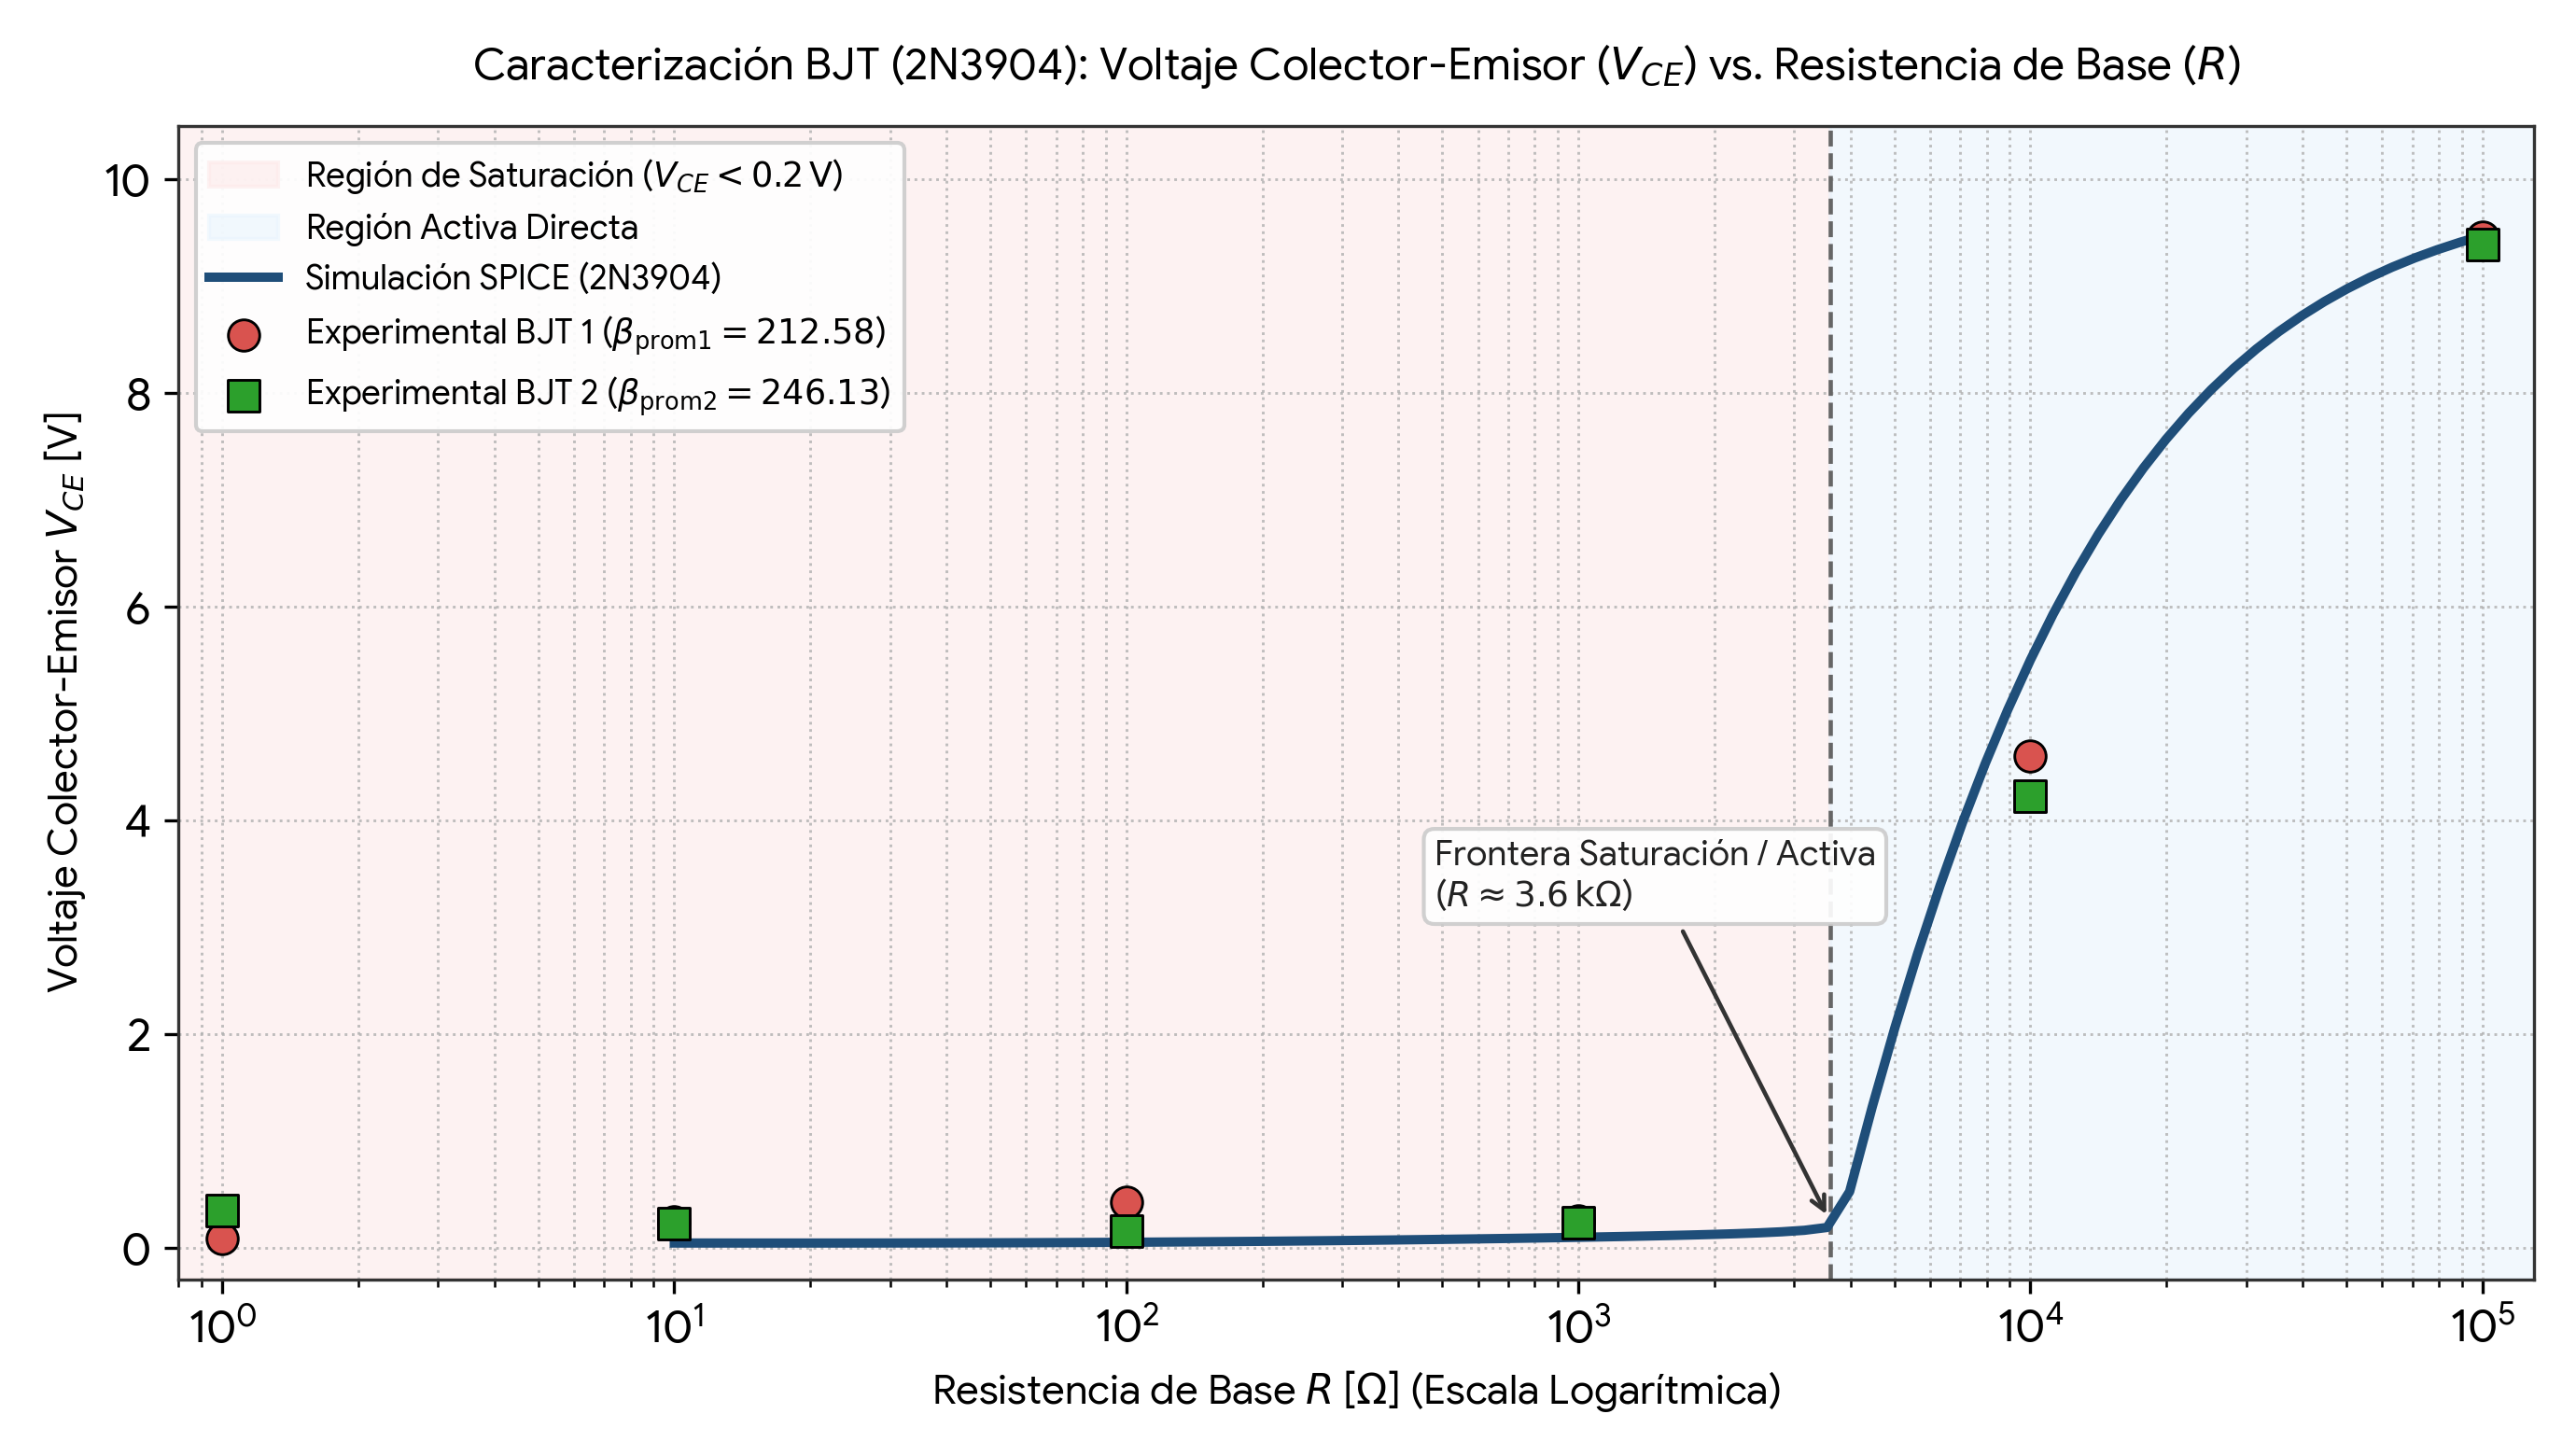
\includegraphics[width=0.86\linewidth]{grafica1_VCE_vs_R_v2.png}
\caption{Voltaje colector-emisor $V_{CE}$ en funci\'on de la resistencia de base $R$ para el BJT 2N3904 (simulaci\'on SPICE y caracterizaci\'on previa de BJT 1 y BJT 2).}
\label{fig:caract_vce}
\end{figure}

En la Fig. \ref{fig:caract_icib} se observan las corrientes $I_C$ e $I_B$ frente a $R$. En saturaci\'on, $I_C$ permanece en una meseta cercana a $I_{C,\mathrm{sat}} \approx 99.5\text{ mA}$ independientemente del aumento de $I_B$, mientras que en regi\'on activa $I_C$ desciende siguiendo la ley $I_C = \beta I_B$ ($I_C \approx 45\text{ mA}$ en $10\text{ k}\Omega$ y $5.0\text{ mA}$ en $100\text{ k}\Omega$).

\begin{figure}[htbp]
\centering
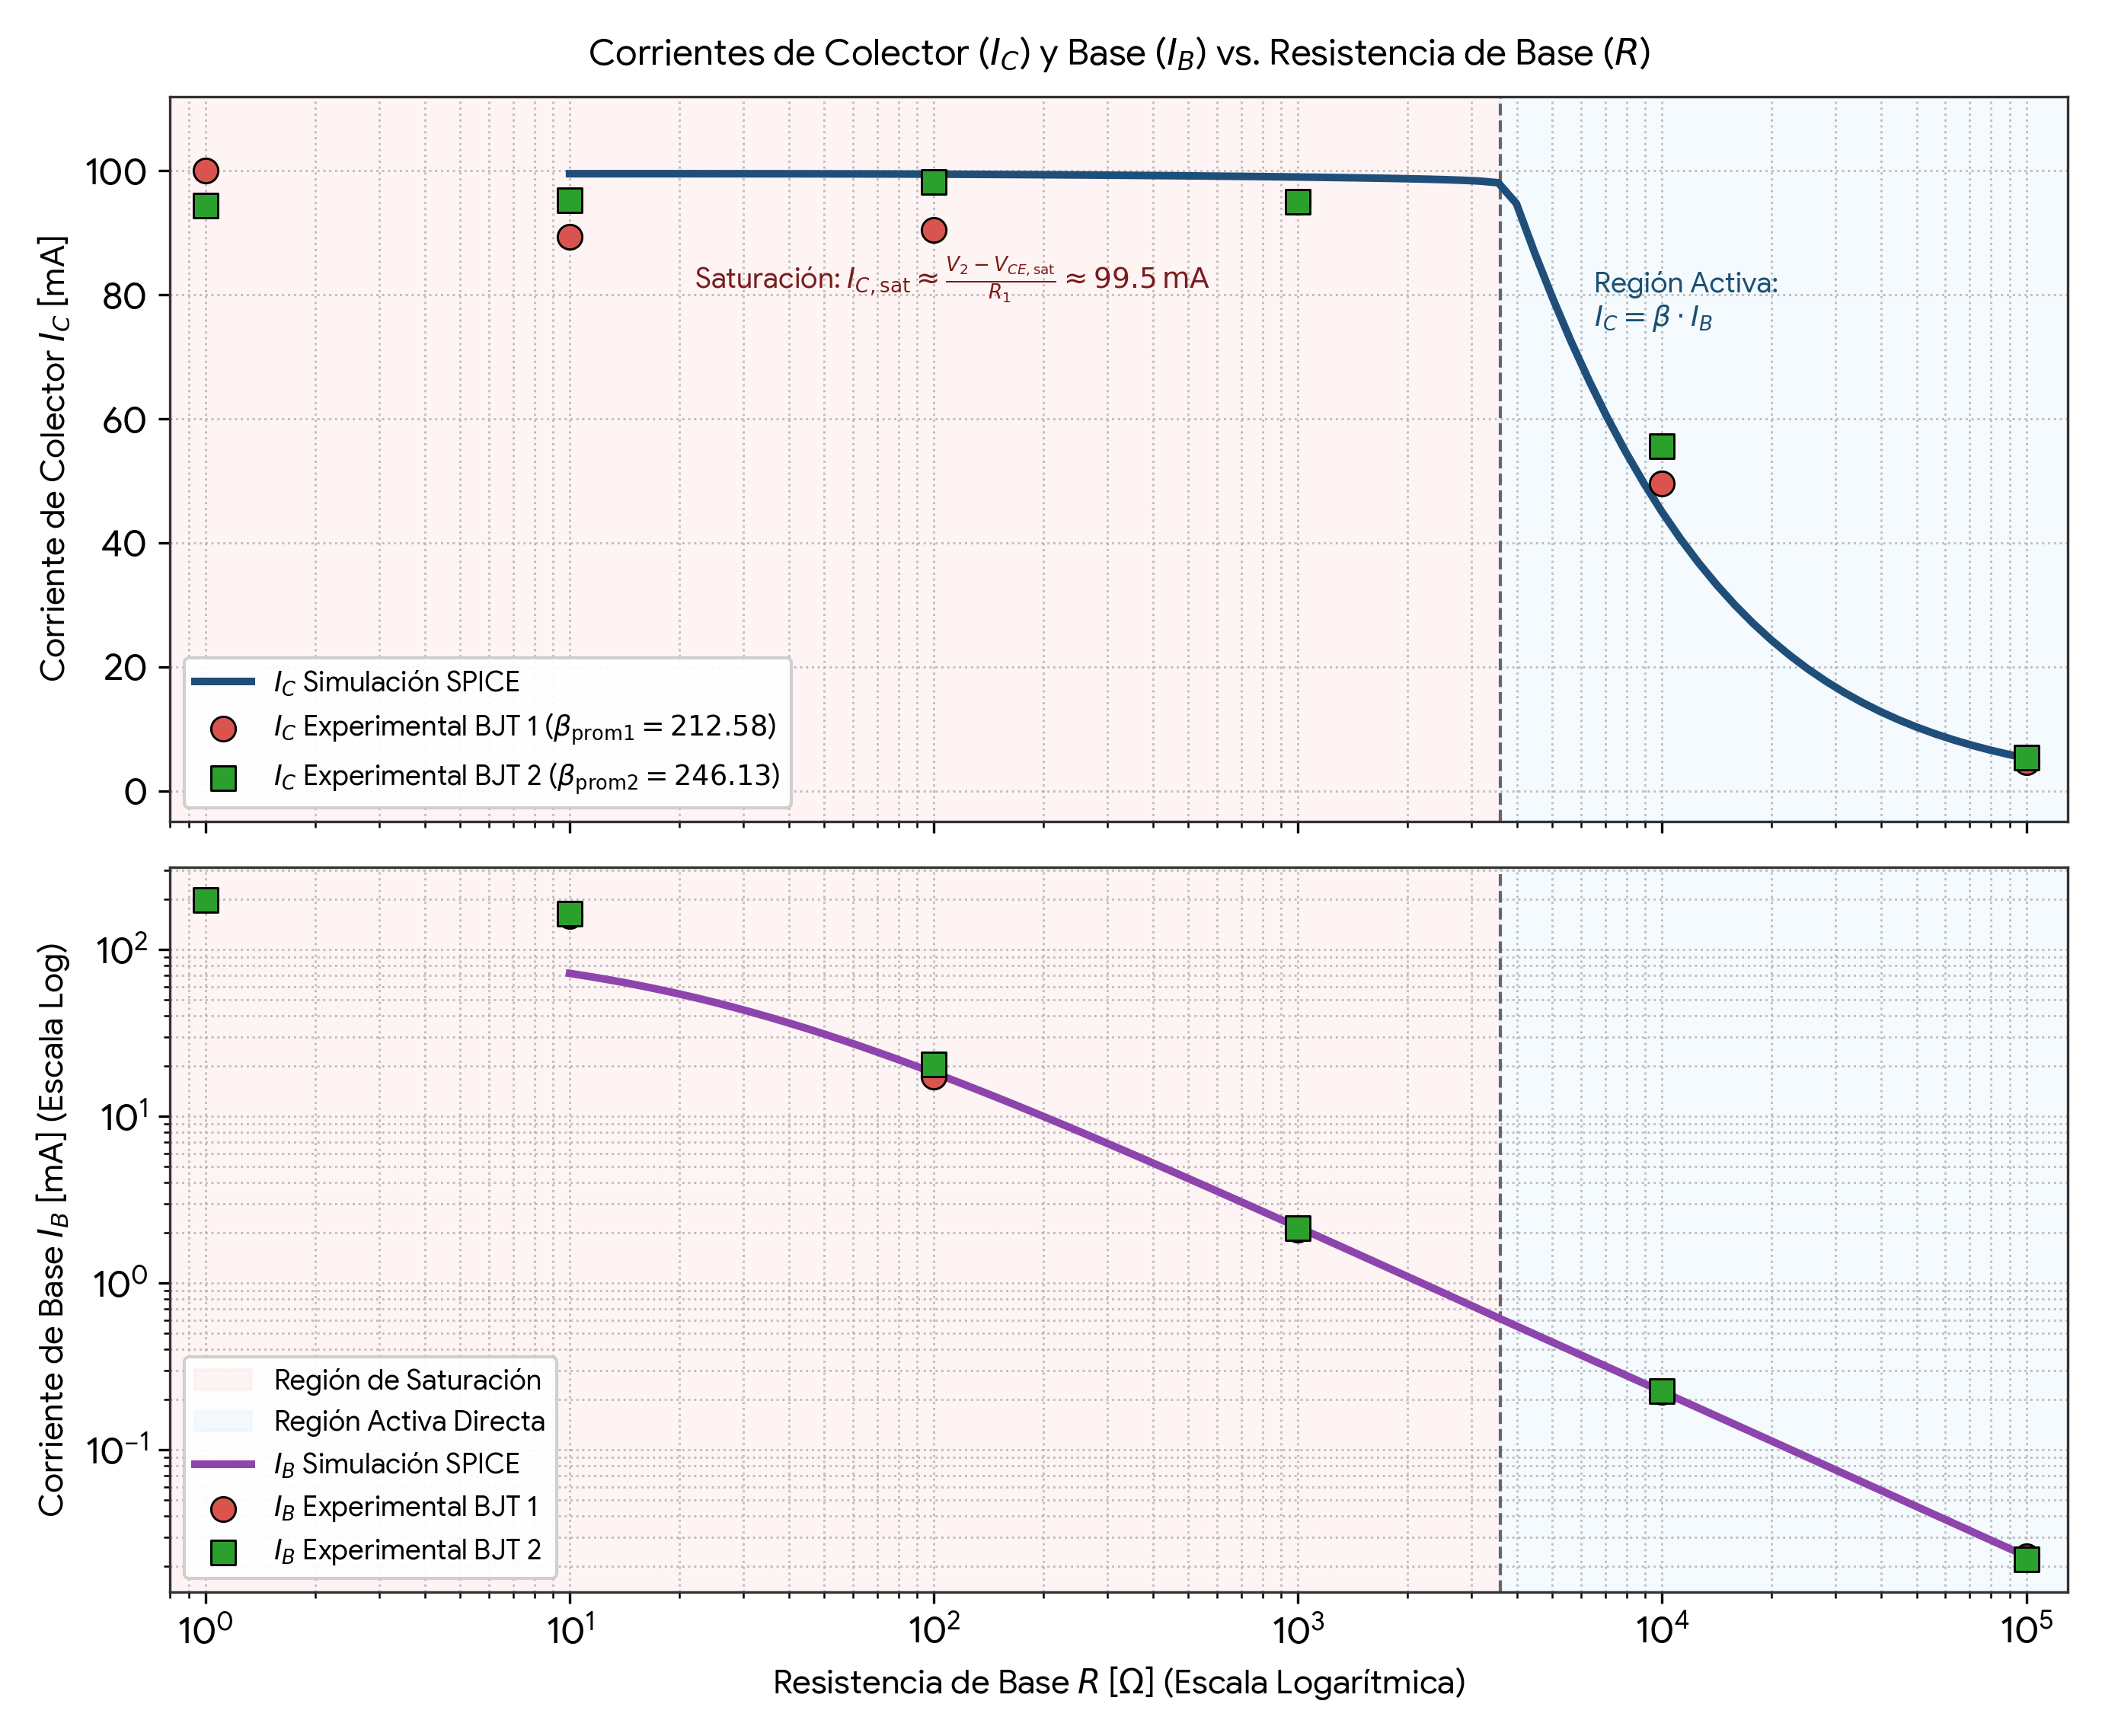
\includegraphics[width=0.82\linewidth]{grafica2_IC_IB_vs_R_v2.png}
\caption{Corrientes de colector $I_C$ y de base $I_B$ en funci\'on de $R$ en escala logar\'itmica.}
\label{fig:caract_icib}
\end{figure}

La Fig. \ref{fig:caract_beta} muestra la curva de transferencia de ganancia de corriente $\beta = I_C/I_B$ en funci\'on de $V_{CE}$. En saturaci\'on se evidencia la ca\'ida dr\'astica de la ganancia forzada ($\beta_{\mathrm{forzado}}$), mientras que en la regi\'on activa la curva simulada asciende gradualmente de $171.33$ a $228.47$ por el efecto Early. Asimismo, los transistores caracterizados registraron promedios en regi\'on activa de $\beta_{\mathrm{prom1}} = 212.58$ (BJT~1) y $\beta_{\mathrm{prom2}} = 246.13$ (BJT~2).

\begin{figure}[htbp]
\centering
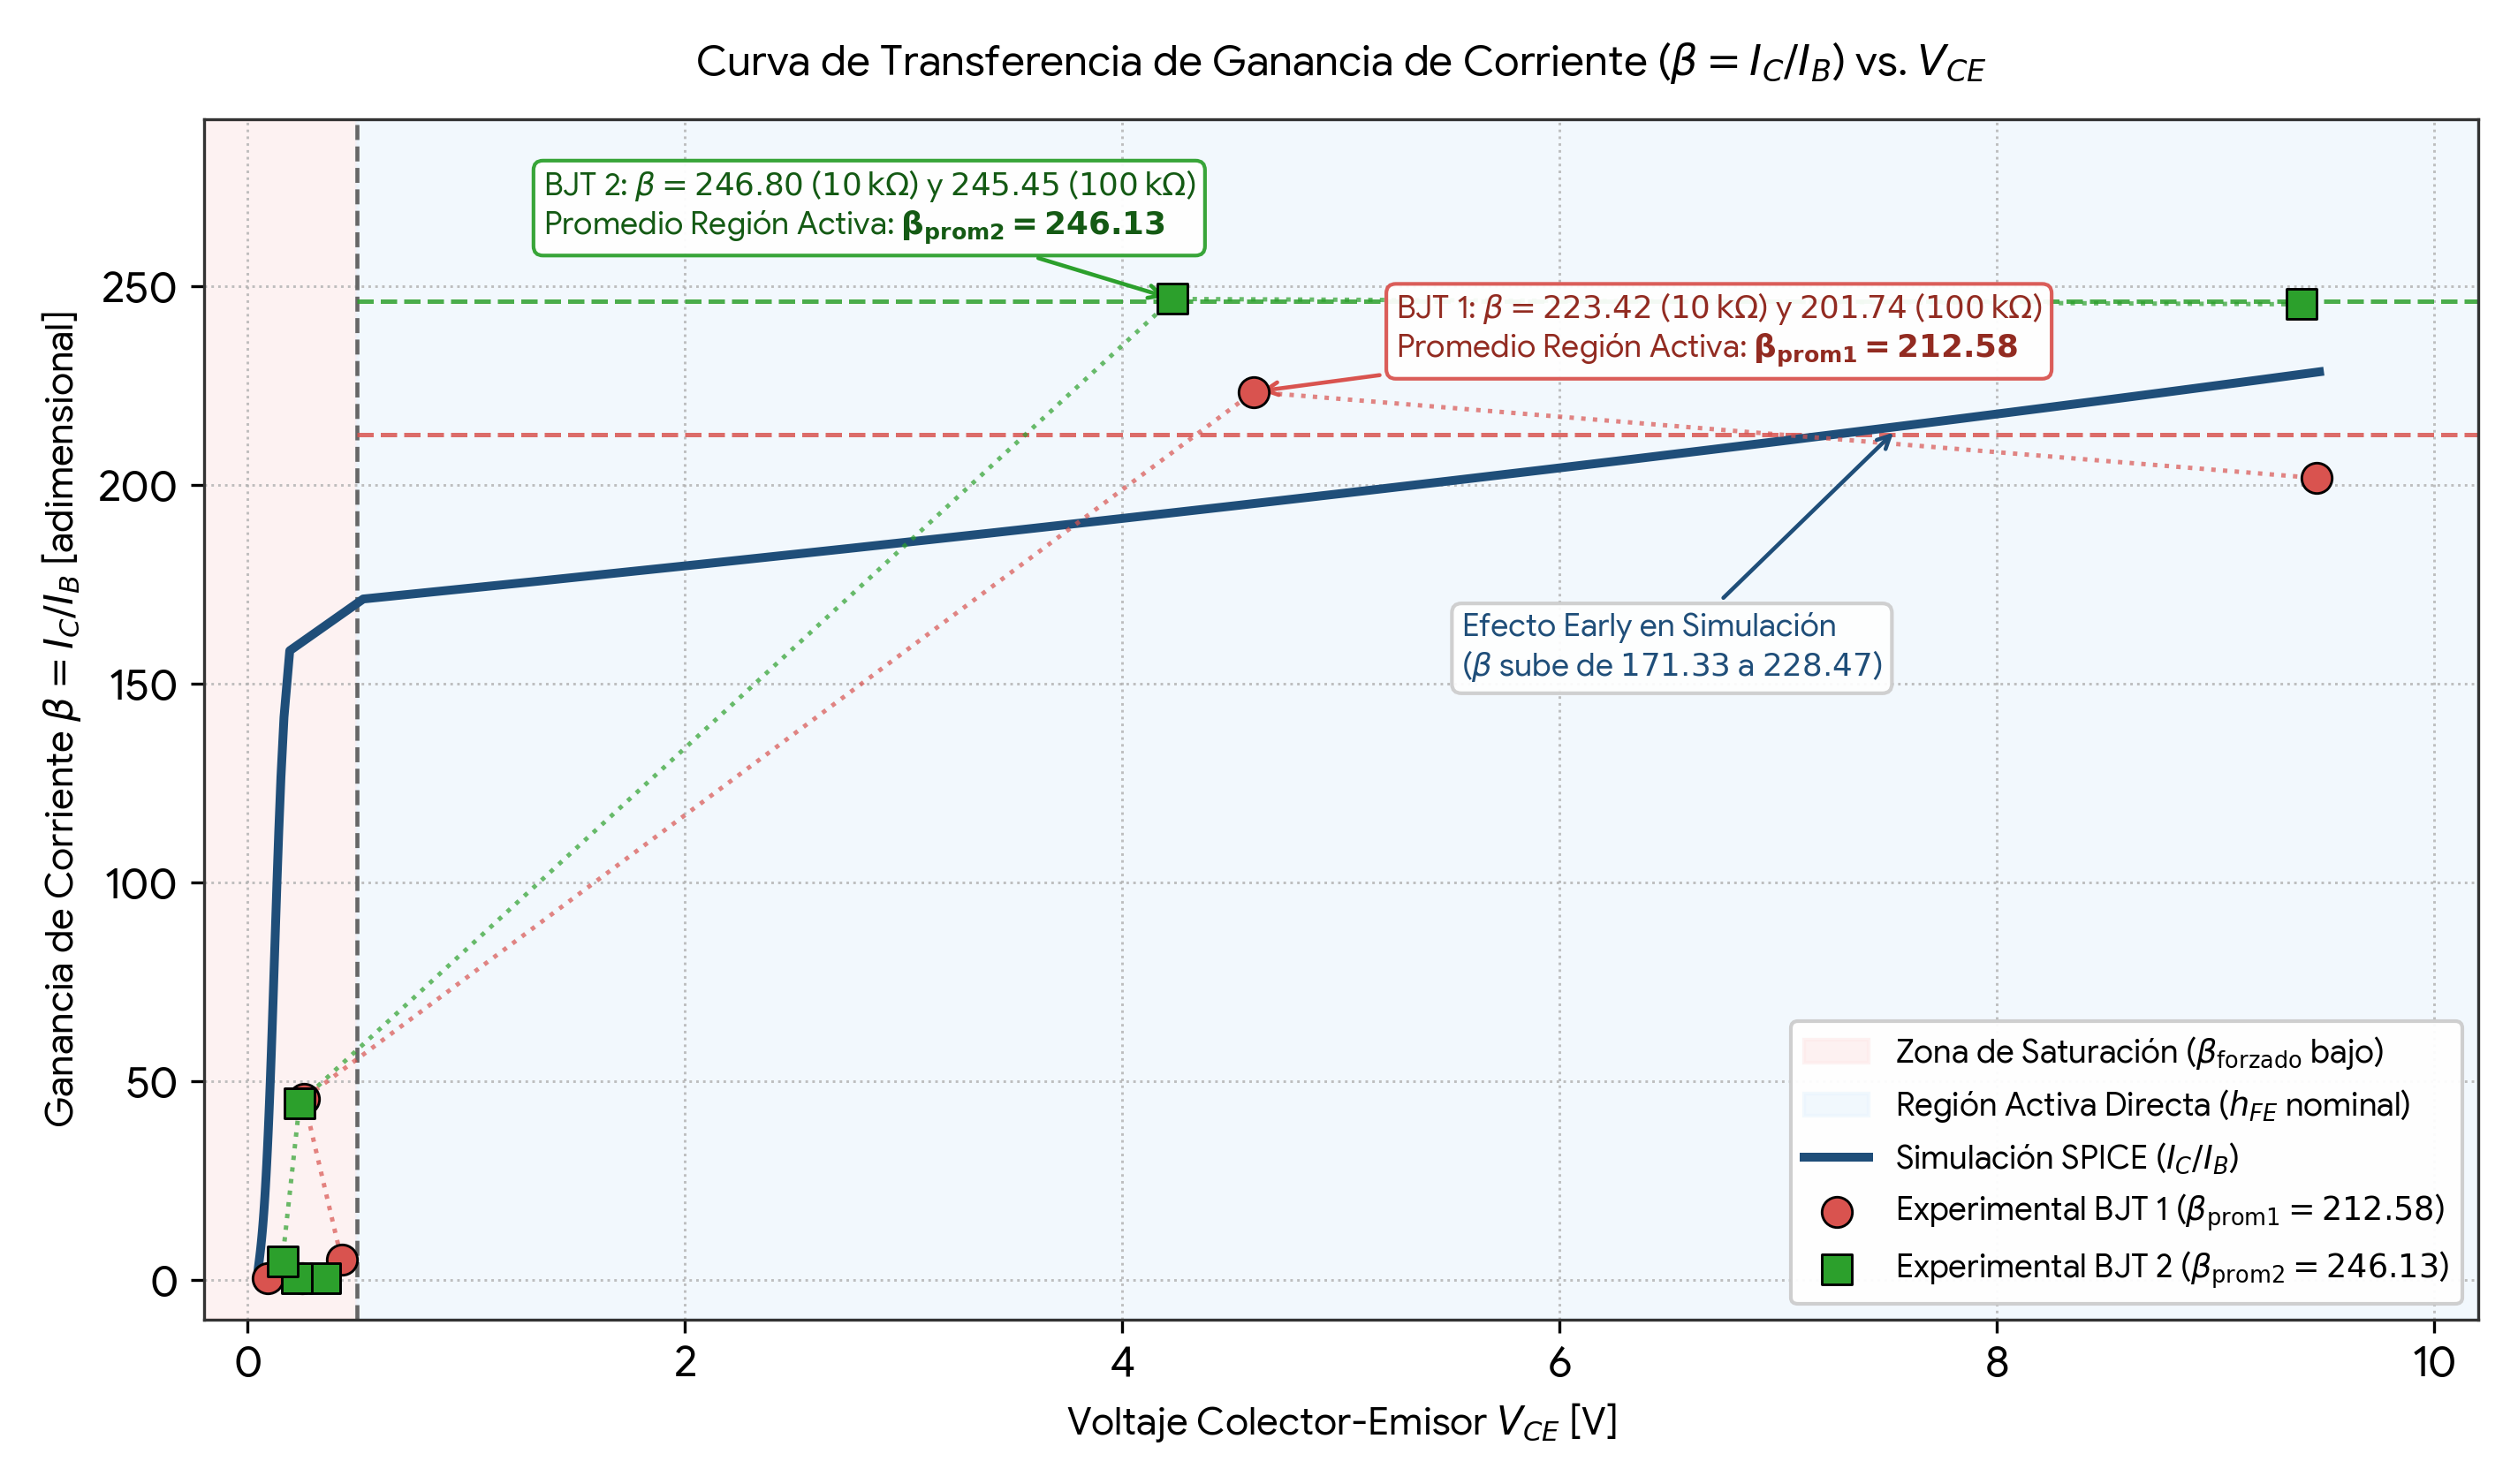
\includegraphics[width=0.86\linewidth]{grafica3_Beta_vs_VCE_v2.png}
\caption{Curva de transferencia de ganancia de corriente $\beta = I_C/I_B$ en funci\'on de $V_{CE}$, evidenciando el efecto Early y los promedios en regi\'on activa.}
\label{fig:caract_beta}
\end{figure}

% =========================================================================
% COMPAÑERO (EMISOR COMÚN): DESCOMENTAR E INTEGRAR LAS GRÁFICAS EXPORTADAS
% DE SIMULACIÓN DE LA CONFIGURACIÓN EMISOR COMÚN INDIVIDUAL.
% =========================================================================
% \subsection{Amplificador en configuraci\'on emisor com\'un}
% % USUARIO (COMPAÑERO): Insertar aquí las gráficas exportadas de LTspice/Python
% % para la respuesta transitoria (Av), impedancia de entrada (Zin), curva de
% % transferencia (Vout vs. Vin) y diagrama de Bode de magnitud del emisor común.
% % \begin{figure}[htbp]
% % \centering
% % \includegraphics[width=0.84\linewidth]{EmisorComun_Av.png}
% % \caption{Respuesta transitoria de entrada y salida del emisor com\'un.}
% % \label{fig:ec_av}
% % \end{figure}
% % \begin{figure}[htbp]
% % \centering
% % \includegraphics[width=0.84\linewidth]{EmisorComun_Transferencia.png}
% % \caption{Curva de transferencia $V_{\mathrm{out}}$ vs. $V_{\mathrm{in}}$ del emisor com\'un.}
% % \label{fig:ec_trans}
% % \end{figure}
% % \begin{figure}[htbp]
% % \centering
% % \includegraphics[width=0.84\linewidth]{EmisorComun_Bode.png}
% % \caption{Diagrama de Bode de magnitud del amplificador emisor com\'un.}
% % \label{fig:ec_bode}
% % \end{figure}

\subsection{Amplificador en configuraci\'on emisor com\'un degenerado}

Para la topolog\'ia de la Fig. \ref{fig:ecd_esq}, la Fig. \ref{fig:ecd_tran} muestra el an\'alisis transitorio a $1\text{ kHz}$ con una entrada senoidal de $50\text{ mV}$ pico y una salida invertida ($180^\circ$) de $195\text{ mV}$ pico, equivalente a $|A_v| = 3.90\text{ V/V}$ ($11.82\text{ dB}$). Las Figs. \ref{fig:ecd_bode_mag} y \ref{fig:ecd_bode_fase} exhiben la respuesta en frecuencia de magnitud y fase, registrando una ganancia en banda media cercana a $11.9\text{ dB}$ (nivel $-3\text{ dB}$ en $8.9\text{ dB}$), fase constante de $180^\circ$ en banda media y frecuencias de corte $f_L \approx 20\text{ Hz}$ y $f_H \approx 10\text{ MHz}$ ($BW \approx 10\text{ MHz}$).

\begin{figure}[htbp]
\centering
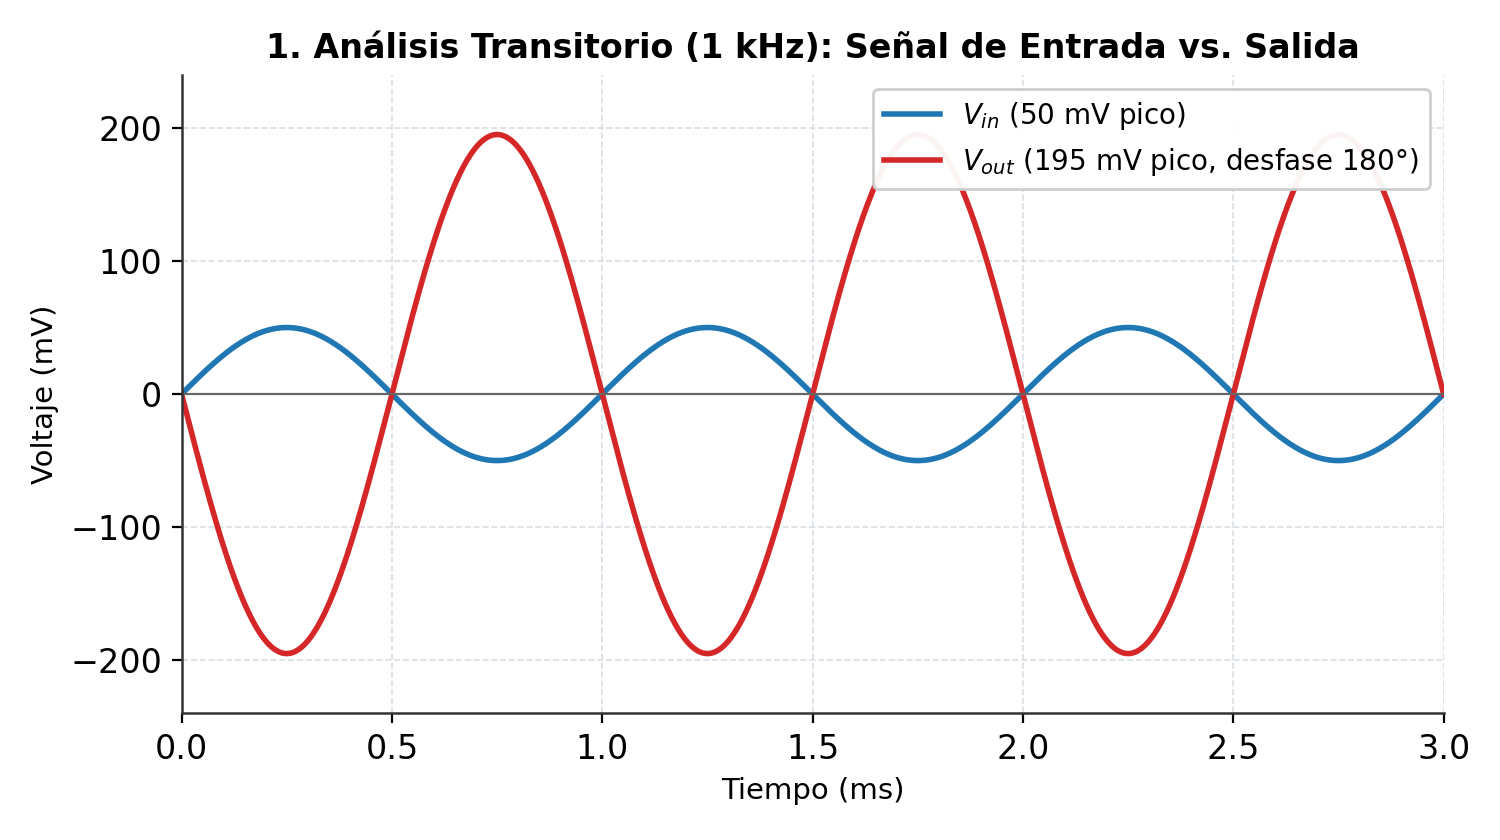
\includegraphics[width=0.84\linewidth]{EmisorDegeneradoVinVout.png}
\caption{Respuesta transitoria de voltaje de entrada y salida para el amplificador emisor com\'un degenerado.}
\label{fig:ecd_tran}
\end{figure}

\begin{figure}[htbp]
\centering
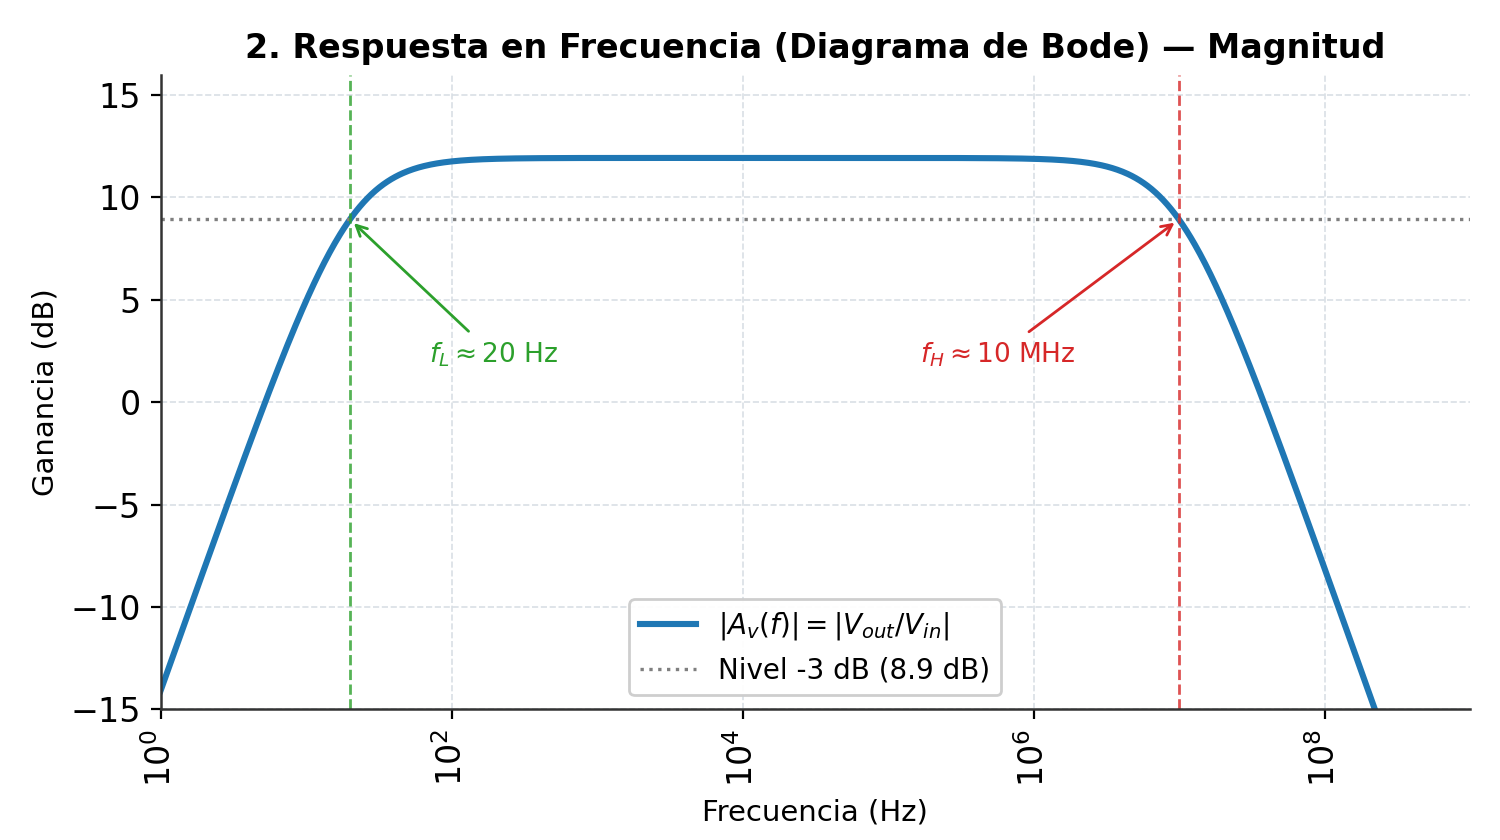
\includegraphics[width=0.84\linewidth]{EmisorDegeneradoBodeMagnitud.png}
\caption{Diagrama de Bode de magnitud del amplificador emisor com\'un degenerado ($f_L \approx 20\text{ Hz}$, $f_H \approx 10\text{ MHz}$).}
\label{fig:ecd_bode_mag}
\end{figure}

\begin{figure}[htbp]
\centering
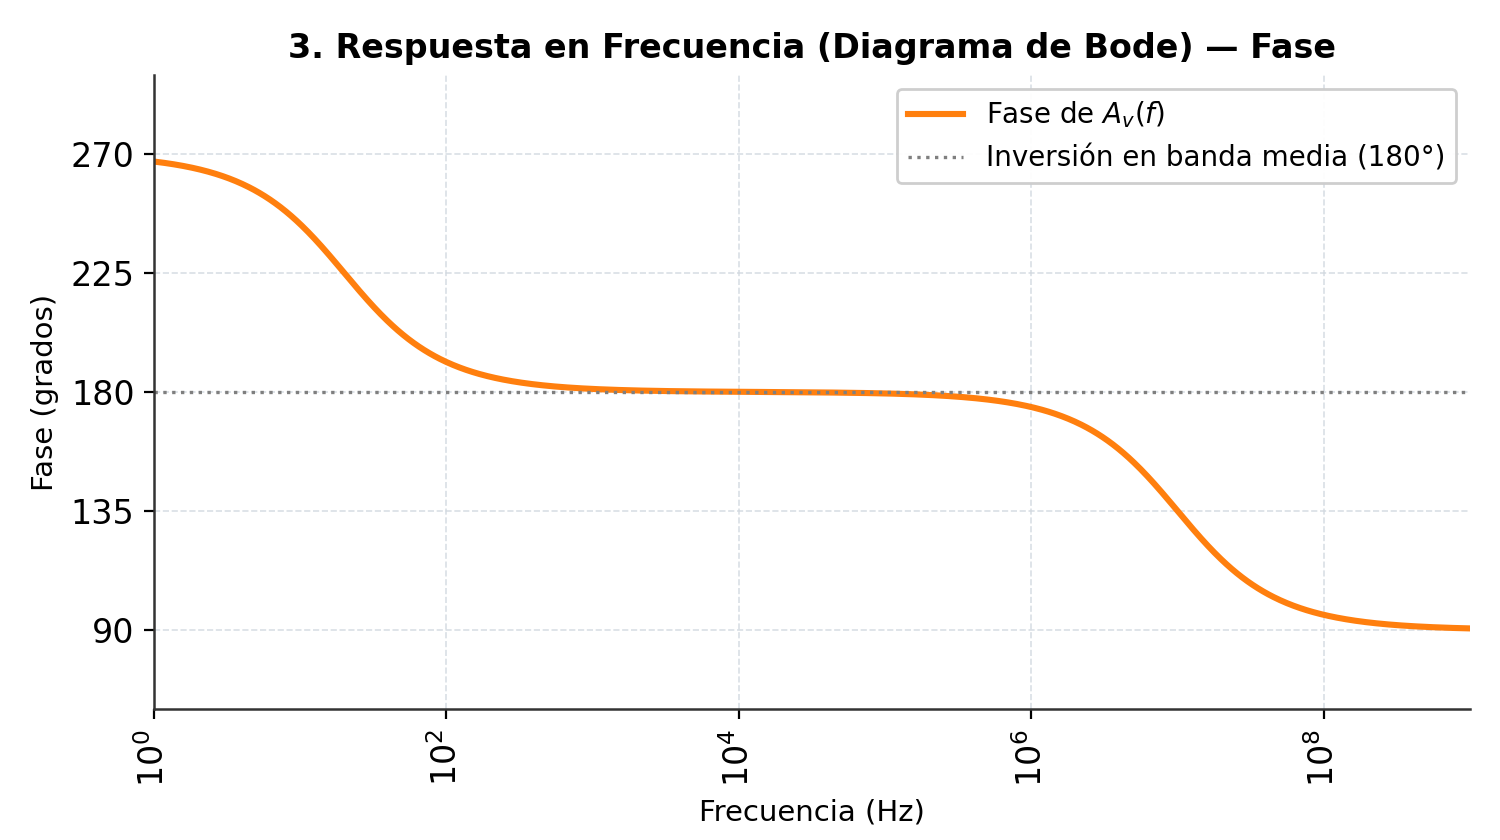
\includegraphics[width=0.84\linewidth]{EmisorDegeneradoBodeFase.png}
\caption{Diagrama de Bode de fase del amplificador emisor com\'un degenerado mostrando la inversi\'on de $180^\circ$ en banda media.}
\label{fig:ecd_bode_fase}
\end{figure}

La medici\'on simulada de impedancia de entrada se ilustra en la Fig. \ref{fig:ecd_zin}, donde $V_{\mathrm{in}} = 50\text{ mV}$ pico e $I_{\mathrm{in}} = 5.0\ \mu\text{A}$ pico en fase arrojan $Z_{\mathrm{in}} = 10.00\text{ k}\Omega$. En la Fig. \ref{fig:ecd_zout} se compara la salida sin carga ($V_{\mathrm{oc}} \approx 238\text{ mV}$ pico) frente a la salida con carga $R_L = 10\text{ k}\Omega$ ($V_L \approx 191\text{ mV}$ pico), de donde se obtiene $Z_{\mathrm{out}} = R_L(V_{\mathrm{oc}}/V_L - 1) \approx 2.46\text{ k}\Omega$. Finalmente, la Fig. \ref{fig:ecd_clip} presenta la condici\'on de sobreexcitaci\'on y recorte, evidenciando l\'imites de excursi\'on de $+5.2\text{ V}$ (superior) y $-5.0\text{ V}$ (inferior).

\begin{figure}[htbp]
\centering
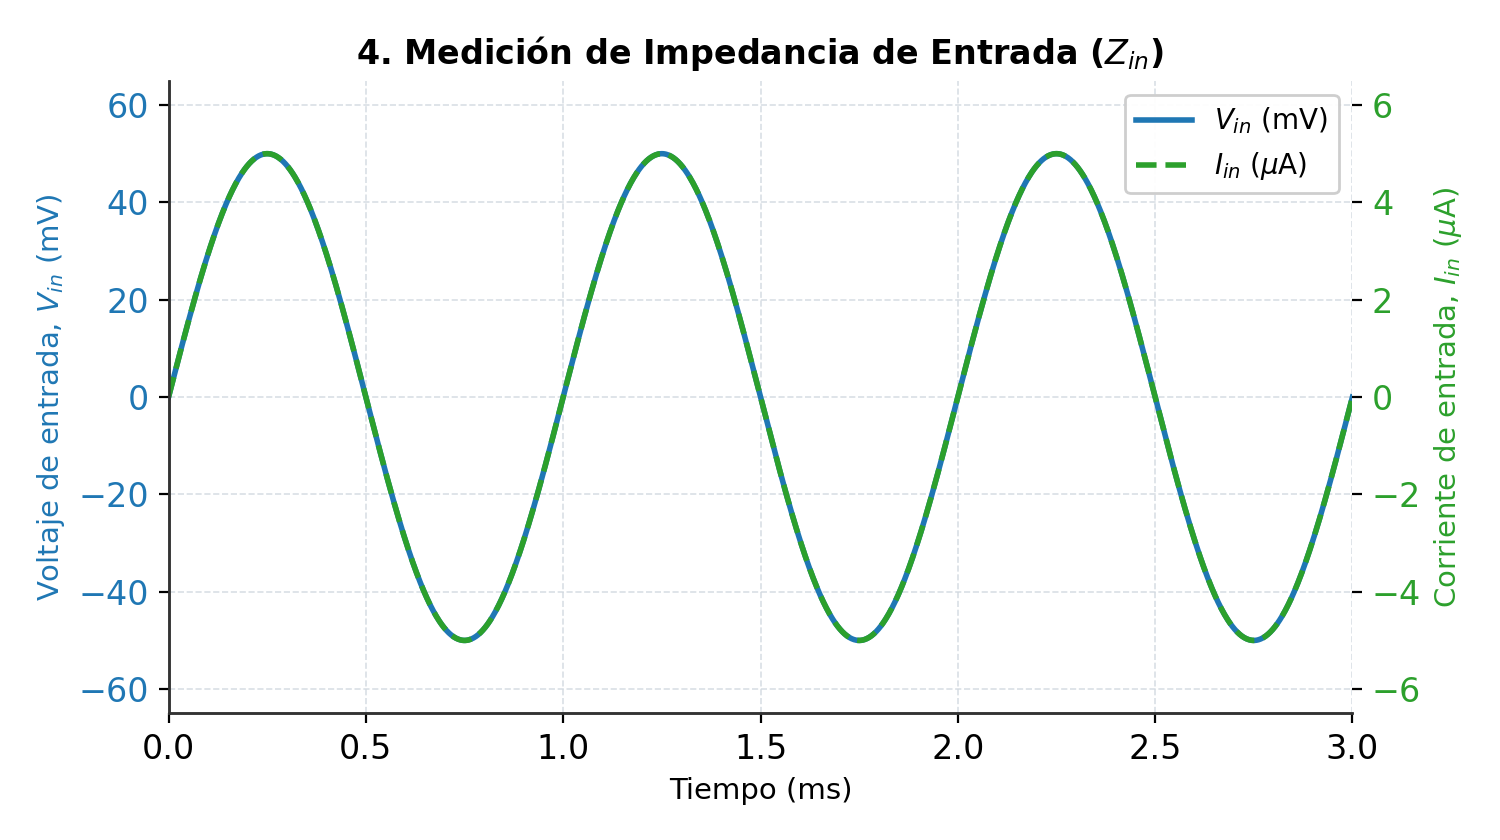
\includegraphics[width=0.84\linewidth]{EmisorDegeneradoZin.png}
\caption{Simulaci\'on de voltaje y corriente de entrada para determinar $Z_{\mathrm{in}}$ en el emisor com\'un degenerado.}
\label{fig:ecd_zin}
\end{figure}

\begin{figure}[htbp]
\centering
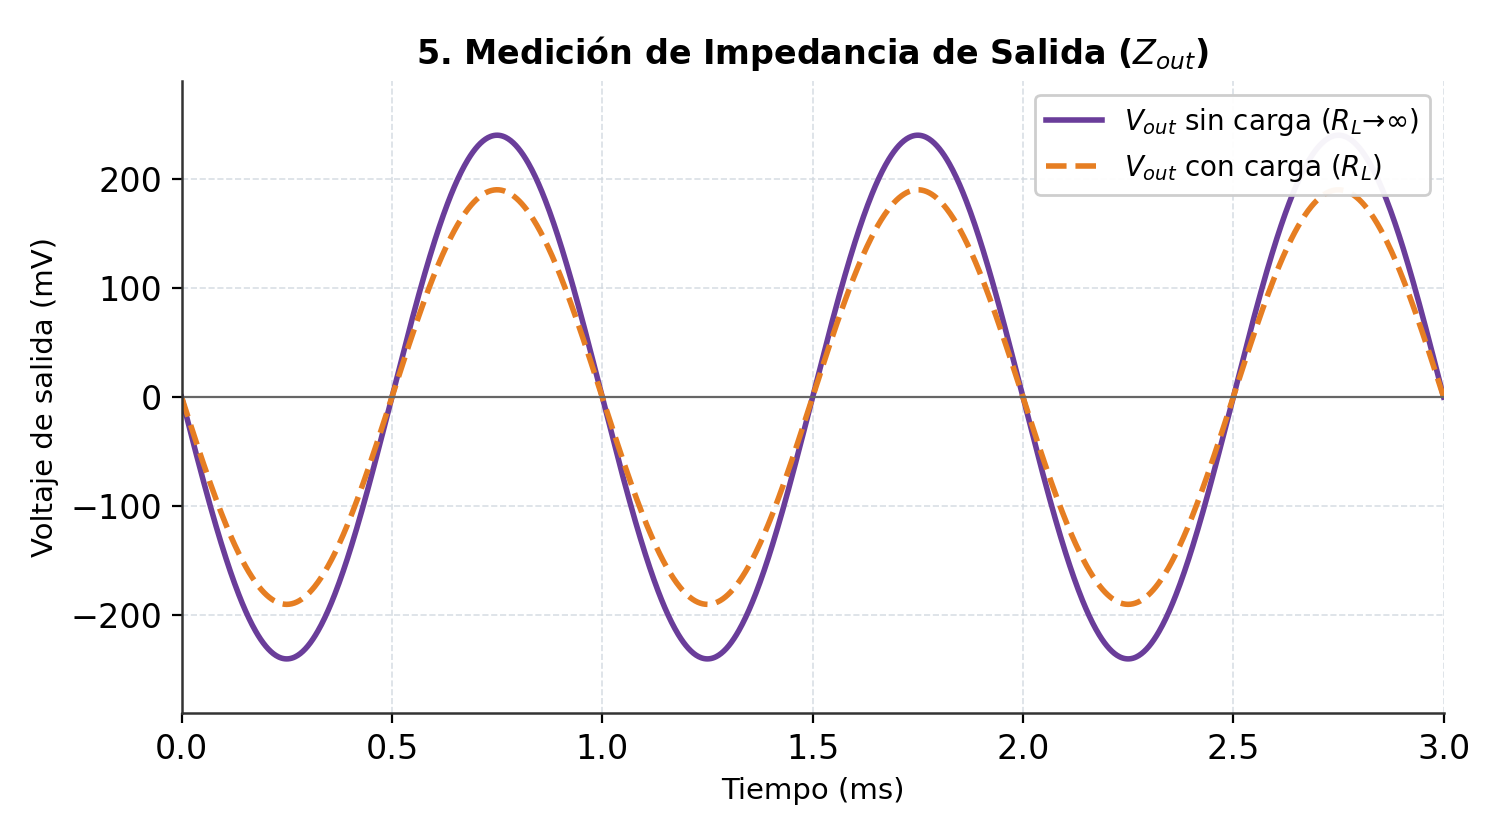
\includegraphics[width=0.84\linewidth]{EmisorDegeneradoZout.png}
\caption{Comparaci\'on de voltaje de salida sin carga y con carga $R_L$ para estimar $Z_{\mathrm{out}}$ en el emisor degenerado.}
\label{fig:ecd_zout}
\end{figure}

\begin{figure}[htbp]
\centering
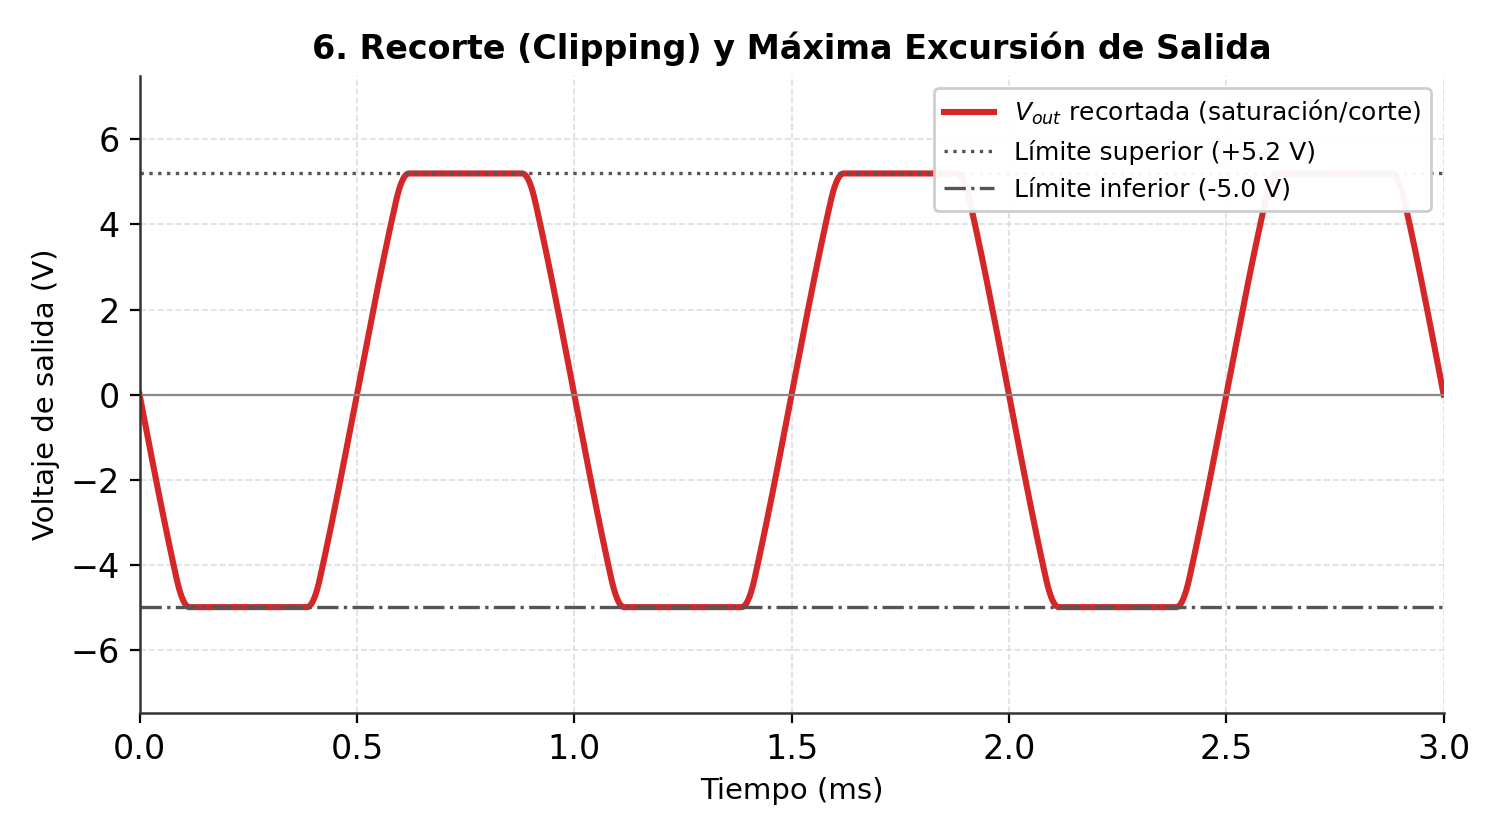
\includegraphics[width=0.84\linewidth]{EmisorDegeneradoRecorteExcursion.png}
\caption{Recorte por saturaci\'on y corte en la salida del emisor com\'un degenerado (l\'imites $+5.2\text{ V}$ y $-5.0\text{ V}$).}
\label{fig:ecd_clip}
\end{figure}

% USUARIO: Si se exporta la curva de transferencia Vout vs. Vin del emisor
% degenerado, descomentar el siguiente bloque e insertar el archivo PNG/JPG.
% \begin{figure}[htbp]
% \centering
% 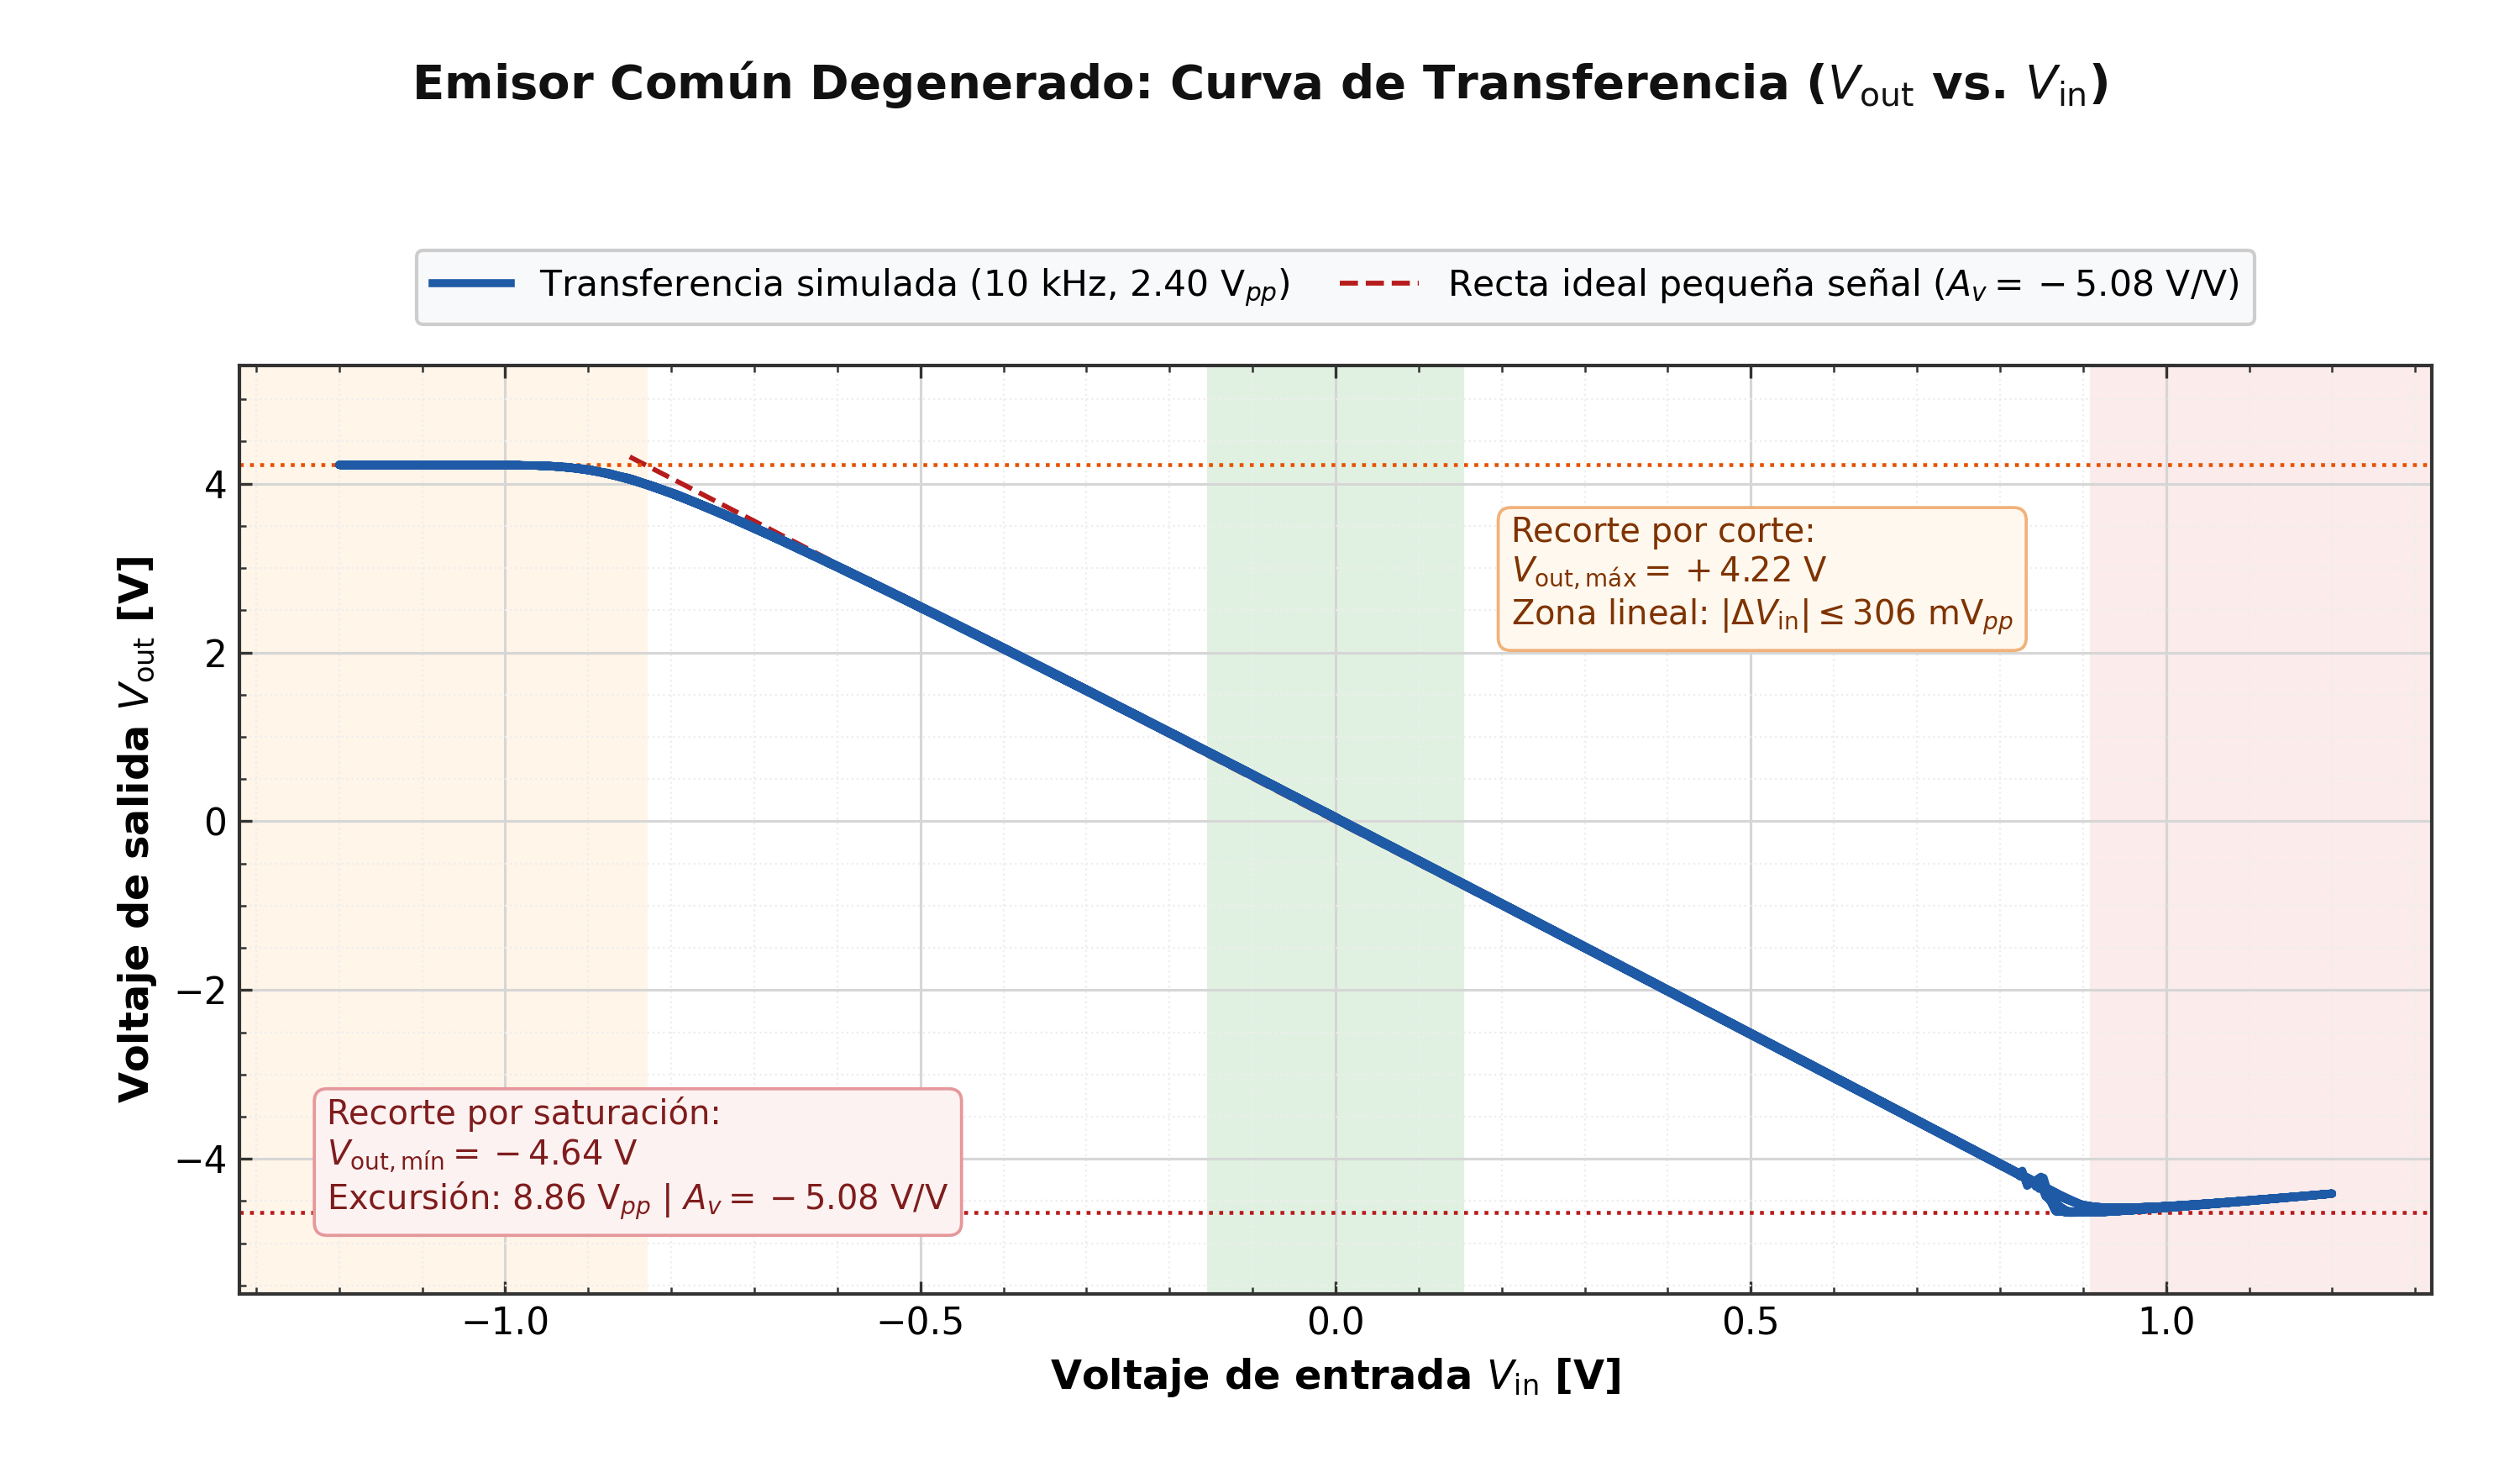
\includegraphics[width=0.84\linewidth]{EmisorDegeneradoTransferencia.png}
% \caption{Curva de transferencia $V_{\mathrm{out}}$ vs. $V_{\mathrm{in}}$ del amplificador emisor com\'un degenerado.}
% \label{fig:ecd_trans}
% \end{figure}

\subsection{Amplificador en configuraci\'on colector com\'un}

Para el seguidor de emisor de la Fig. \ref{fig:cc_esq}, la respuesta transitoria a $10\text{ kHz}$ con $V_{\mathrm{in}} = 100\text{ mV}$ pico ($200\text{ mV}_{pp}$) se muestra en la Fig. \ref{fig:cc_tran}, obteni\'endose $V_{\mathrm{out}} \approx 98\text{ mV}$ pico ($A_v \approx 0.980\text{ V/V}$) sin inversi\'on de fase ($\Delta\phi \approx 0^\circ$). Las Figs. \ref{fig:cc_bode_mag} y \ref{fig:cc_bode_fase} confirman una ganancia plana de $-0.20\text{ dB}$ en banda media, fase nula en la banda de paso, frecuencia de corte inferior $f_L \approx 10.5\text{ Hz}$ (donde la fase alcanza $+45^\circ$) y una frecuencia de corte superior por encima de $100\text{ MHz}$.

\begin{figure}[htbp]
\centering
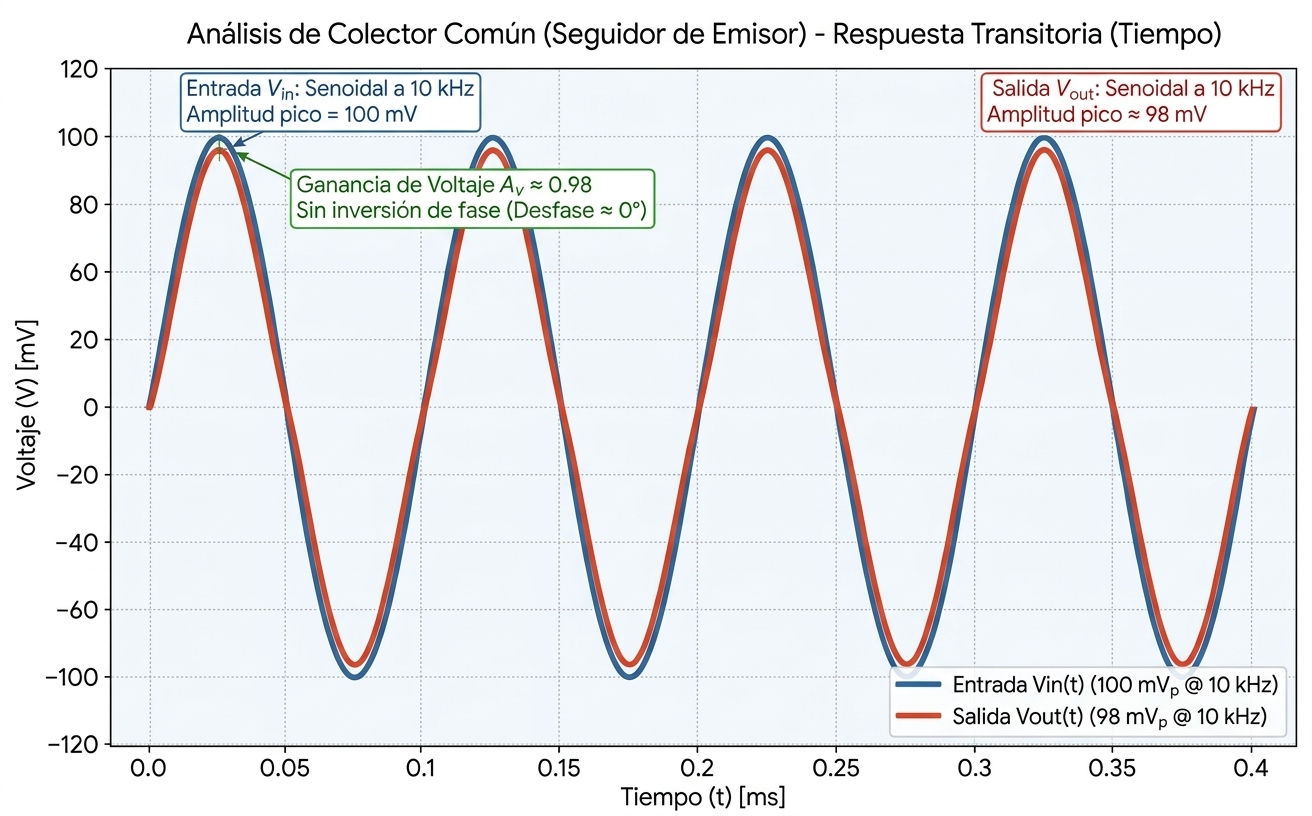
\includegraphics[width=0.84\linewidth]{ColectorComunRespuestaTransitoria.jpg}
\caption{Respuesta transitoria de entrada y salida del amplificador colector com\'un a $10\text{ kHz}$ ($A_v \approx 0.98$, desfase $\approx 0^\circ$).}
\label{fig:cc_tran}
\end{figure}

\begin{figure}[htbp]
\centering
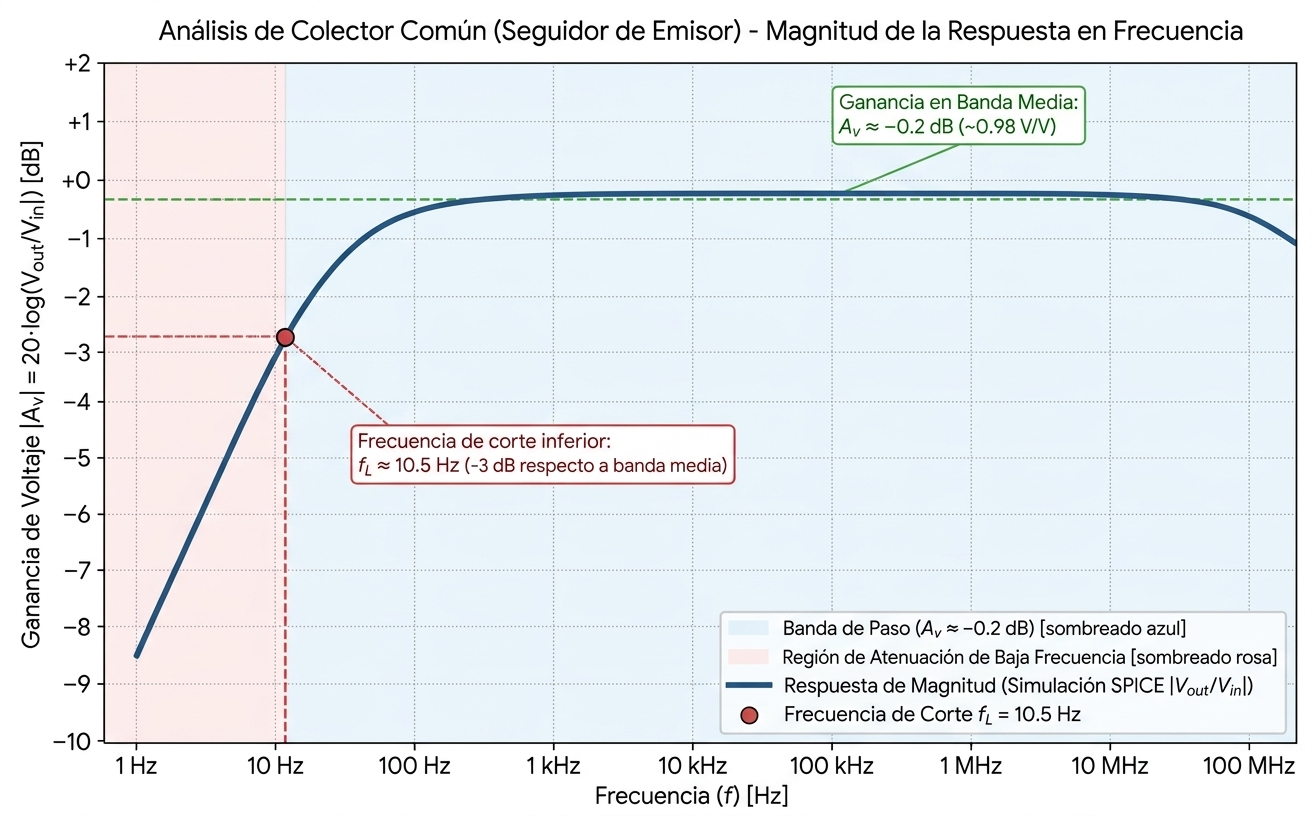
\includegraphics[width=0.84\linewidth]{ColectorComunMagnitudRespuestaFrecuencia.jpg}
\caption{Diagrama de Bode de magnitud del amplificador colector com\'un ($f_L \approx 10.5\text{ Hz}$, banda media $-0.2\text{ dB}$).}
\label{fig:cc_bode_mag}
\end{figure}

\begin{figure}[htbp]
\centering
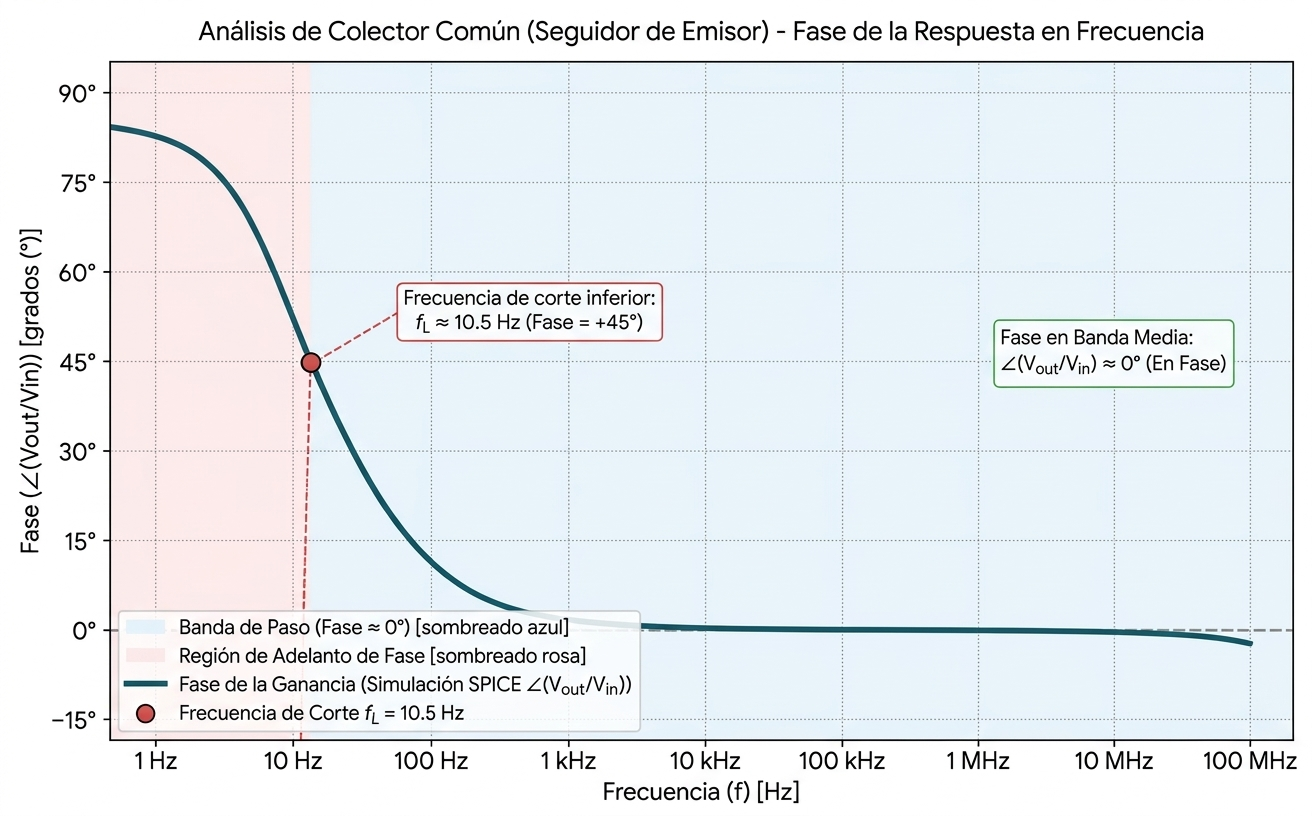
\includegraphics[width=0.84\linewidth]{ColectorComunFaseRespuestaFrecuencia.jpg}
\caption{Diagrama de Bode de fase del amplificador colector com\'un mostrando adelanto de $+45^\circ$ en $f_L \approx 10.5\text{ Hz}$.}
\label{fig:cc_bode_fase}
\end{figure}

% USUARIO: Inserta aquí las gráficas faltantes de Colector Común (curva de
% transferencia Vout vs. Vin e impedancia de entrada Zin) cuando las exportes
% de LTspice/Python, y descomenta los bloques siguientes.
% \begin{figure}[htbp]
% \centering
% \includegraphics[width=0.84\linewidth]{ColectorComunTransferencia.jpg}
% \caption{Curva de transferencia $V_{\mathrm{out}}$ vs. $V_{\mathrm{in}}$ del amplificador colector com\'un.}
% \label{fig:cc_trans}
% \end{figure}
% \begin{figure}[htbp]
% \centering
% \includegraphics[width=0.84\linewidth]{ColectorComunZin.jpg}
% \caption{Simulaci\'on de impedancia de entrada $Z_{\mathrm{in}}$ del amplificador colector com\'un.}
% \label{fig:cc_zin}
% \end{figure}

\subsection{Amplificador en cascada (EC + CC)}

En el amplificador en cascada de la Fig. \ref{fig:casc_esq}, la Fig. \ref{fig:casc_av} presenta la respuesta transitoria en peque\~na se\~nal a $10\text{ kHz}$ con $V_{\mathrm{in}} = 10.00\text{ mV}_{pp}$, generando una salida limpia e invertida ($180^\circ$) de $V_{\mathrm{out}} = 1.528\text{ V}_{pp}$, lo que corresponde a $|A_v| = 152.78\text{ V/V}$ ($43.68\text{ dB}$).

\begin{figure}[htbp]
\centering
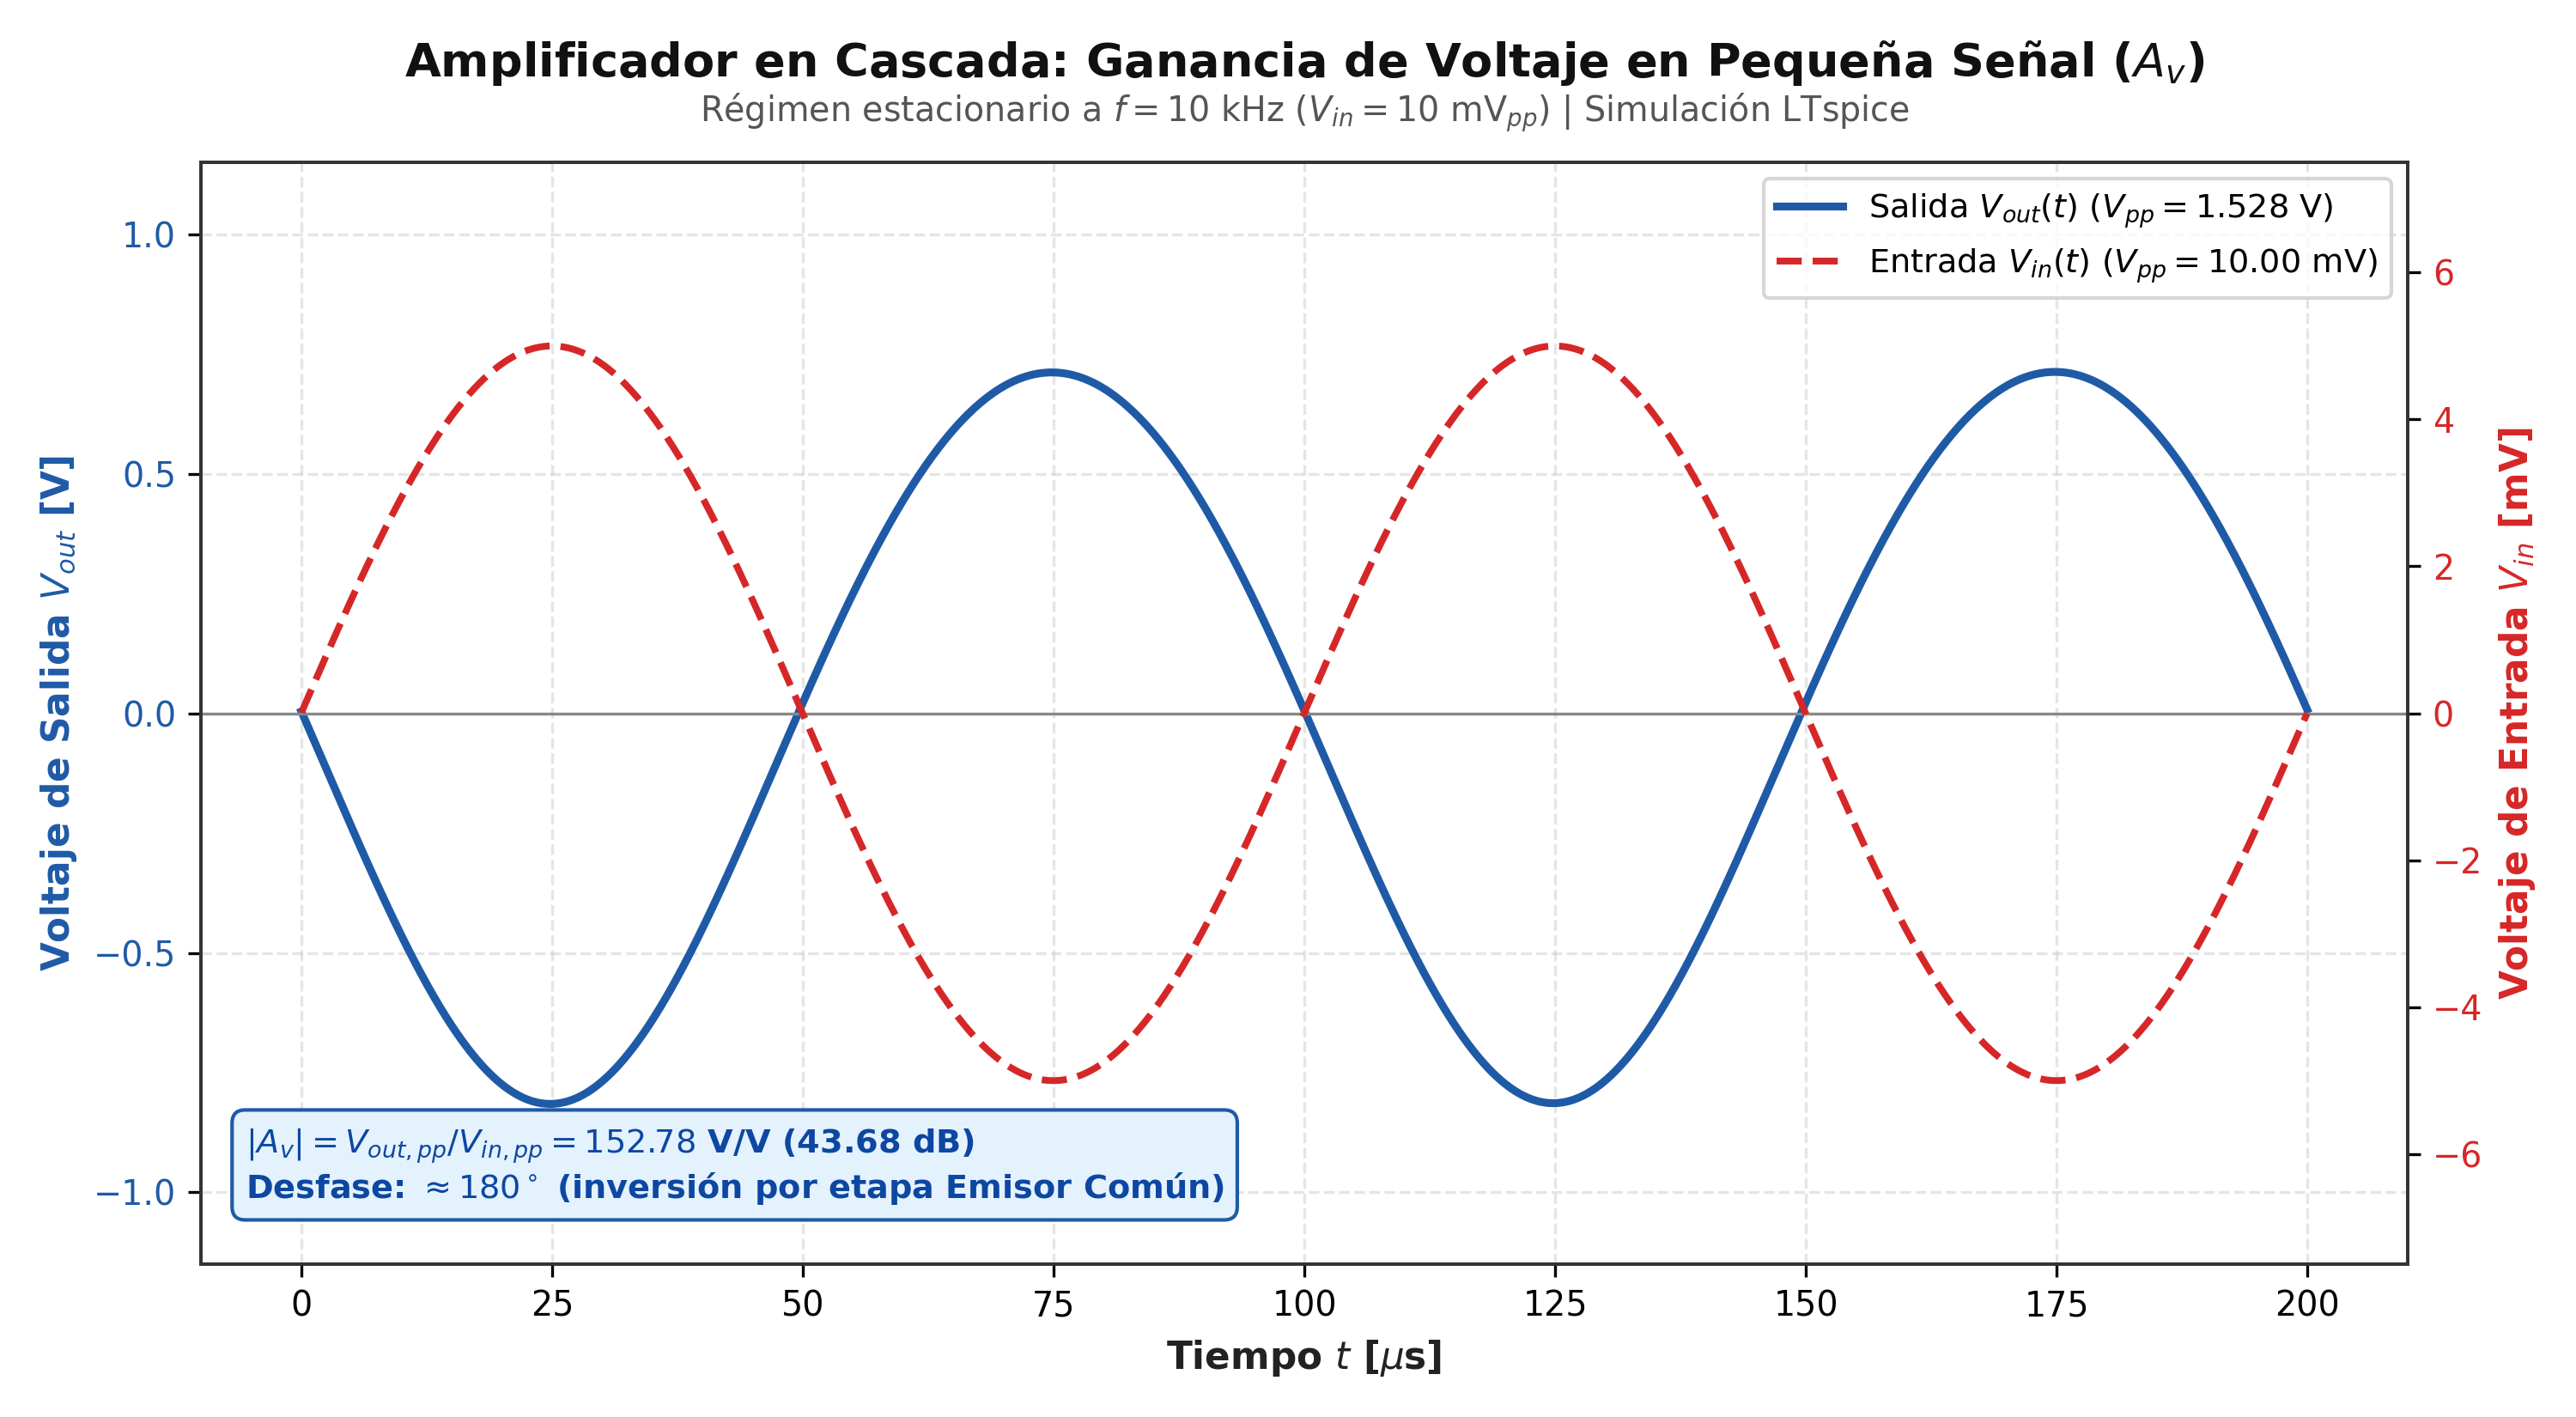
\includegraphics[width=0.84\linewidth]{AmplificadorCascadaAv.png}
\caption{Respuesta transitoria en peque\~na se\~nal del amplificador en cascada a $10\text{ kHz}$ ($|A_v| = 152.78\text{ V/V}$, desfase $180^\circ$).}
\label{fig:casc_av}
\end{figure}

La Fig. \ref{fig:casc_zin} ilustra la obtenci\'on de la impedancia de entrada mediante $V_{\mathrm{in}}(t)$ ($10.00\text{ mV}_{pp}$) e $I_{\mathrm{in}}(t) = -I(C_2)$ ($4.21\ \mu\text{A}_{pp}$), resultando $|Z_{\mathrm{in}}| = 2.37\text{ k}\Omega$ ($2\,373\ \Omega$) con un desfase m\'inimo de $3.4^\circ$. La curva de transferencia de gran se\~nal ($V_{\mathrm{in}} = 200\text{ mV}_{pp}$ a $10\text{ kHz}$) de la Fig. \ref{fig:casc_trans} delimita la regi\'on lineal de peque\~na se\~nal ($\Delta V_{\mathrm{in}} \approx 10\text{ mV}_{pp}$ con pendiente $-152.8\text{ V/V}$) y los l\'imites de recorte en $+4.12\text{ V}$ y $-4.66\text{ V}$. Finalmente, el diagrama de Bode de magnitud de la Fig. \ref{fig:casc_bode} confirma una ganancia en banda media de $43.66\text{ dB}$ ($152.4\text{ V/V}$), frecuencia de corte inferior $f_L = 106.7\text{ Hz}$ y superior $f_H = 9.52\text{ MHz}$, otorgando un ancho de banda $BW = 9.52\text{ MHz}$.

\begin{figure}[htbp]
\centering
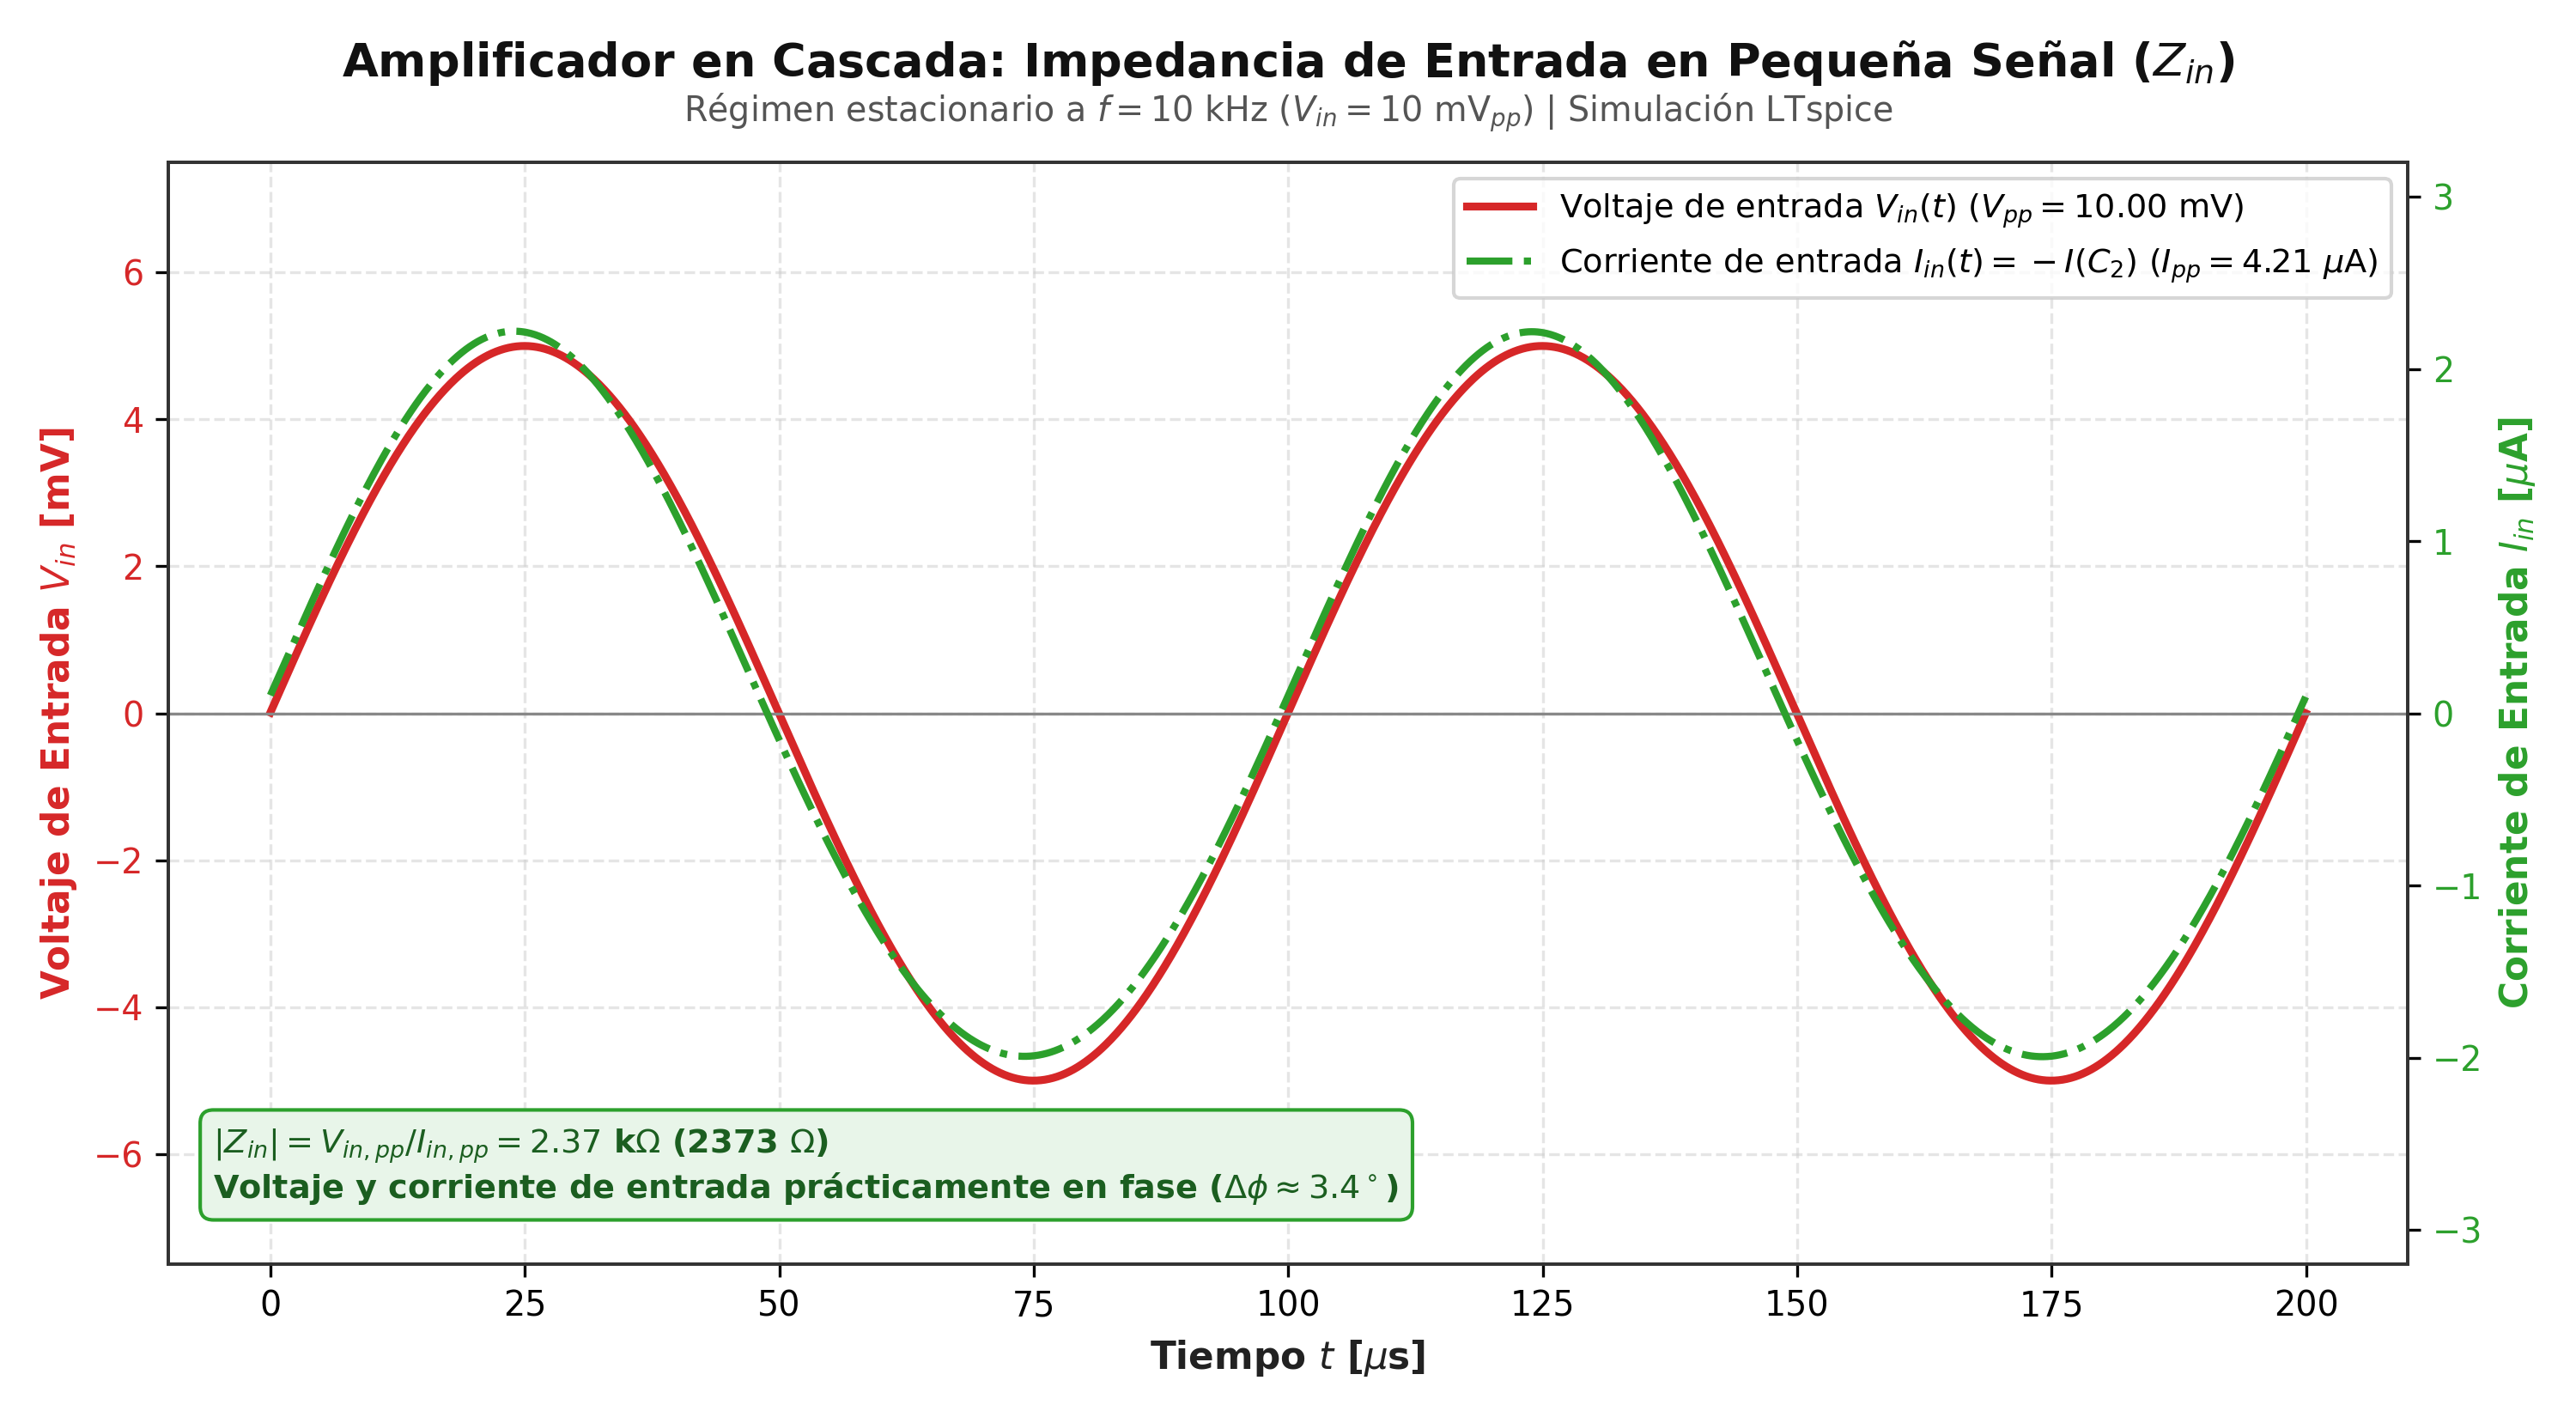
\includegraphics[width=0.84\linewidth]{AmplificadorCascadaZin.png}
\caption{Voltaje y corriente de entrada del amplificador en cascada a $10\text{ kHz}$ ($|Z_{\mathrm{in}}| = 2.37\text{ k}\Omega$).}
\label{fig:casc_zin}
\end{figure}

\begin{figure}[htbp]
\centering
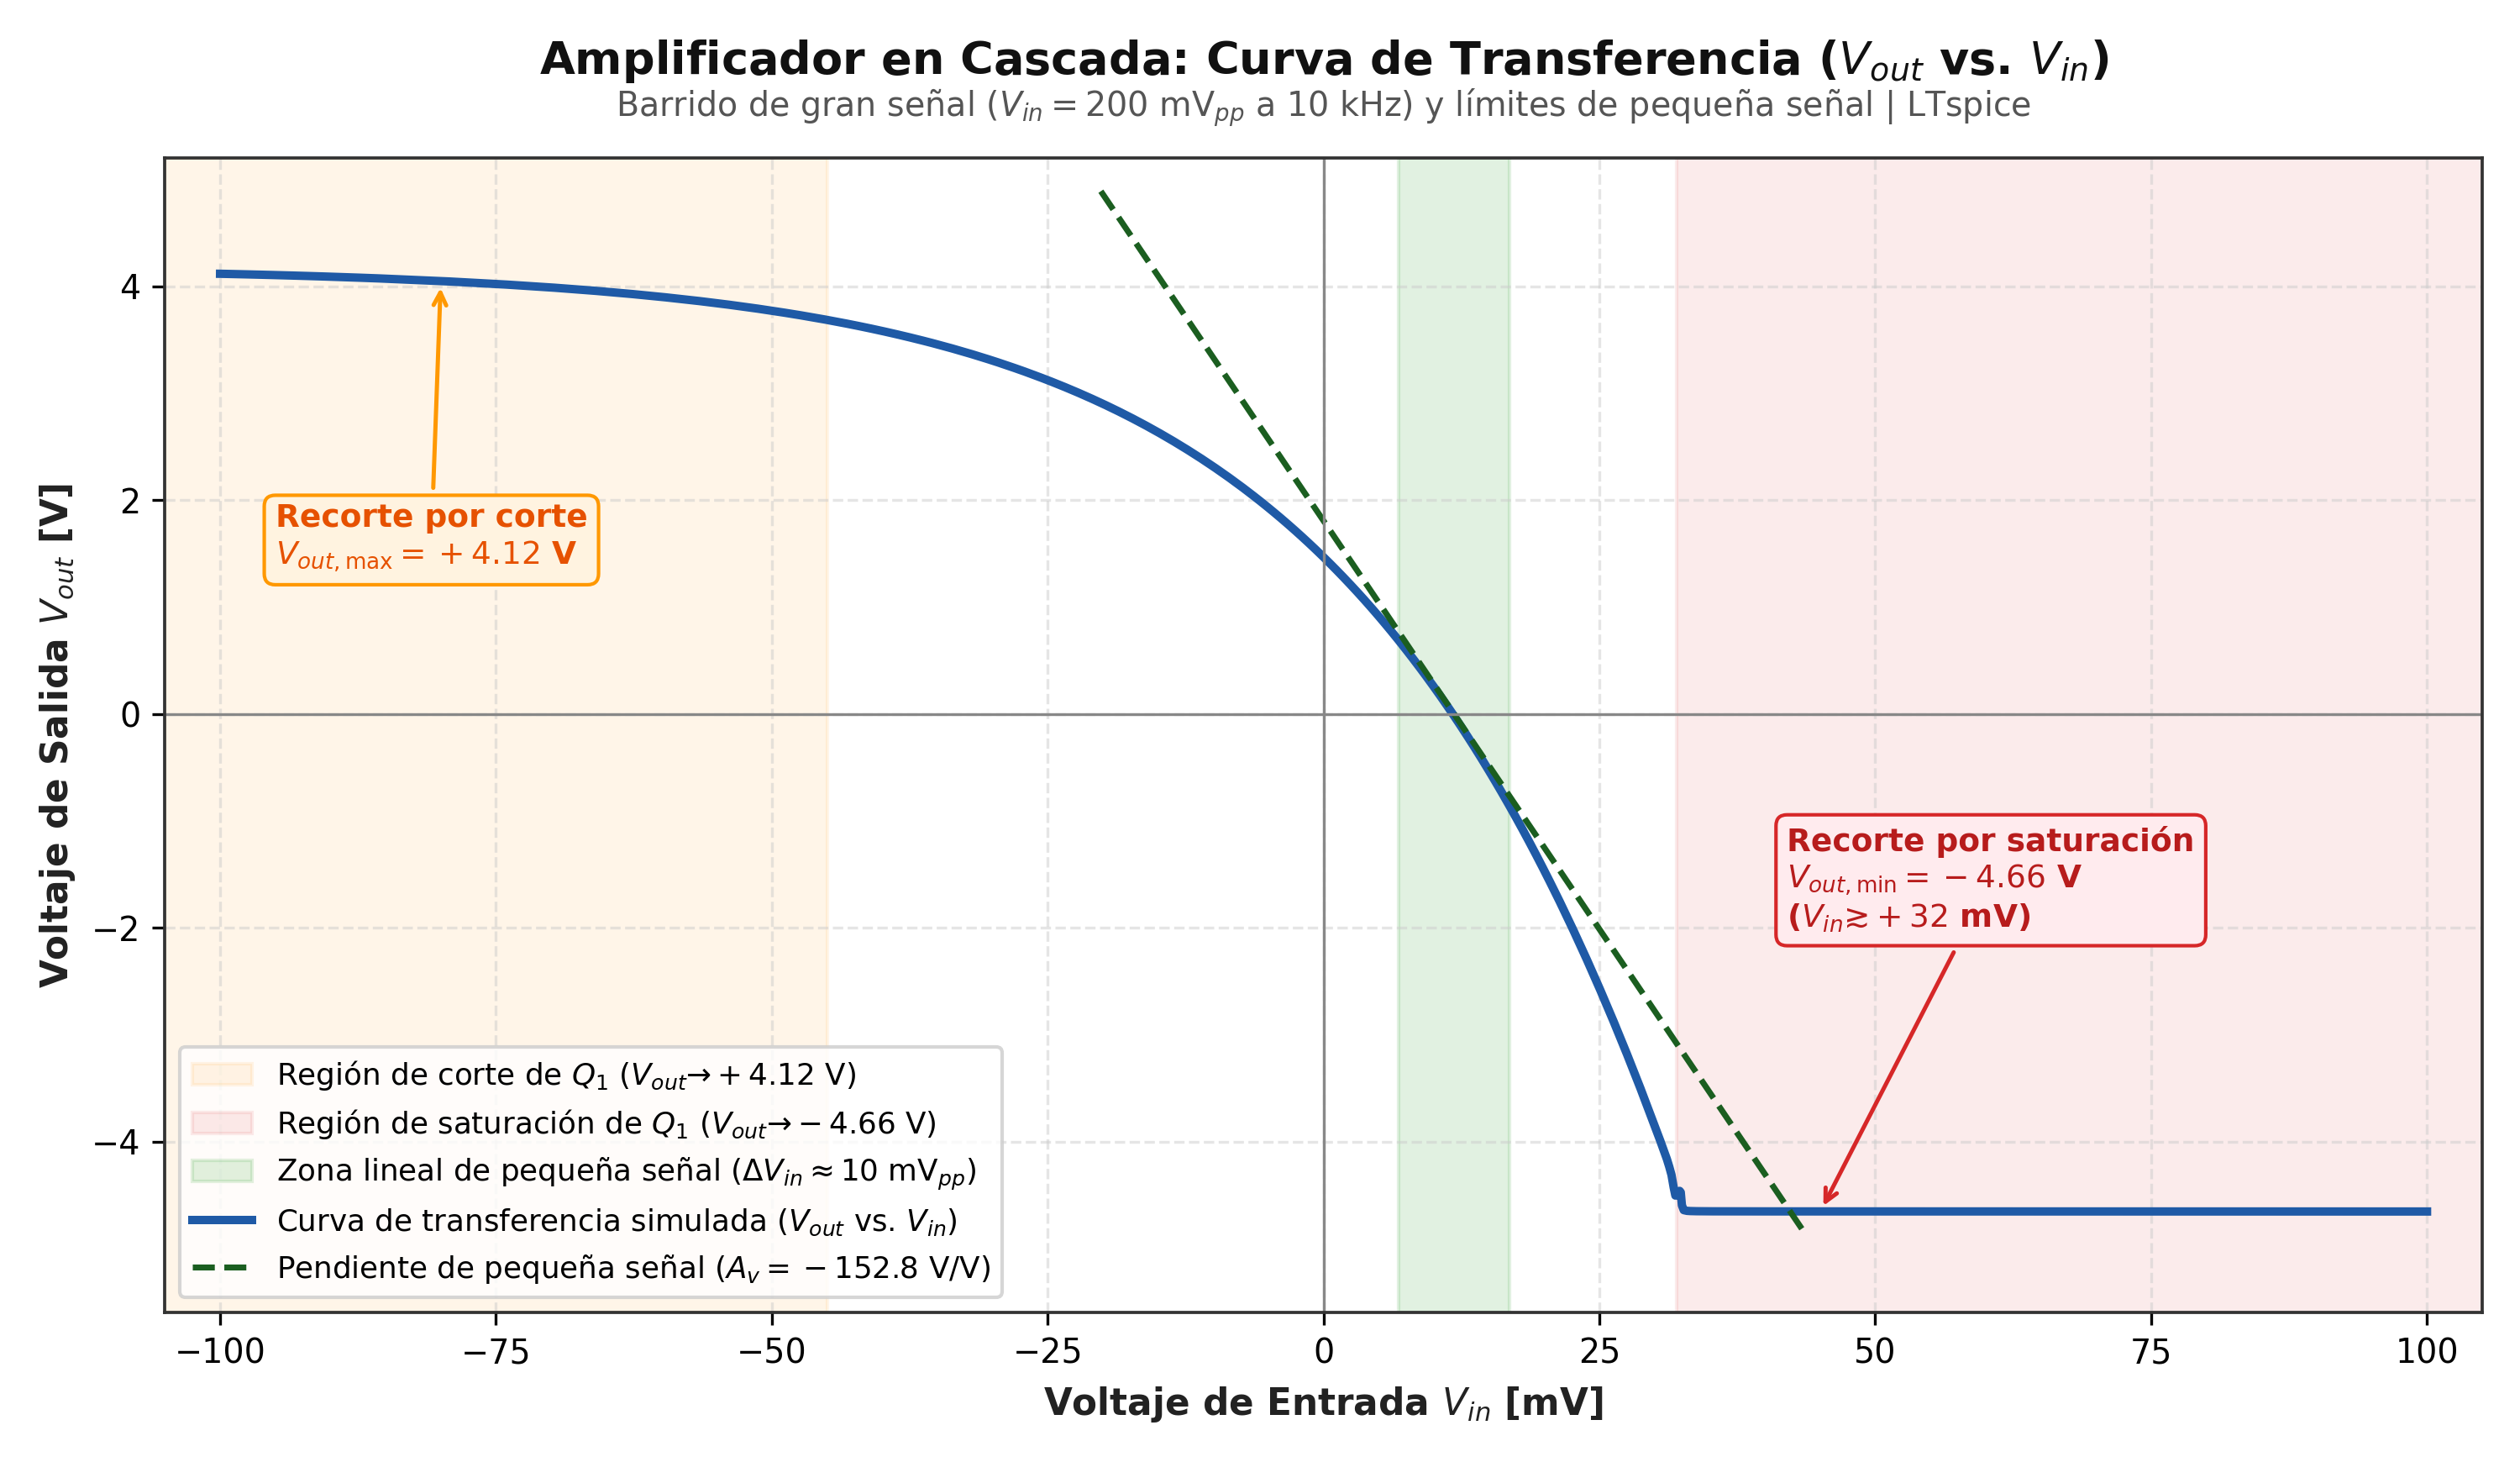
\includegraphics[width=0.84\linewidth]{AmplificadorCascadaTransferencia.png}
\caption{Curva de transferencia $V_{\mathrm{out}}$ vs. $V_{\mathrm{in}}$ del amplificador en cascada, mostrando zona lineal y l\'imites de recorte ($+4.12\text{ V}$ y $-4.66\text{ V}$).}
\label{fig:casc_trans}
\end{figure}

\begin{figure}[htbp]
\centering
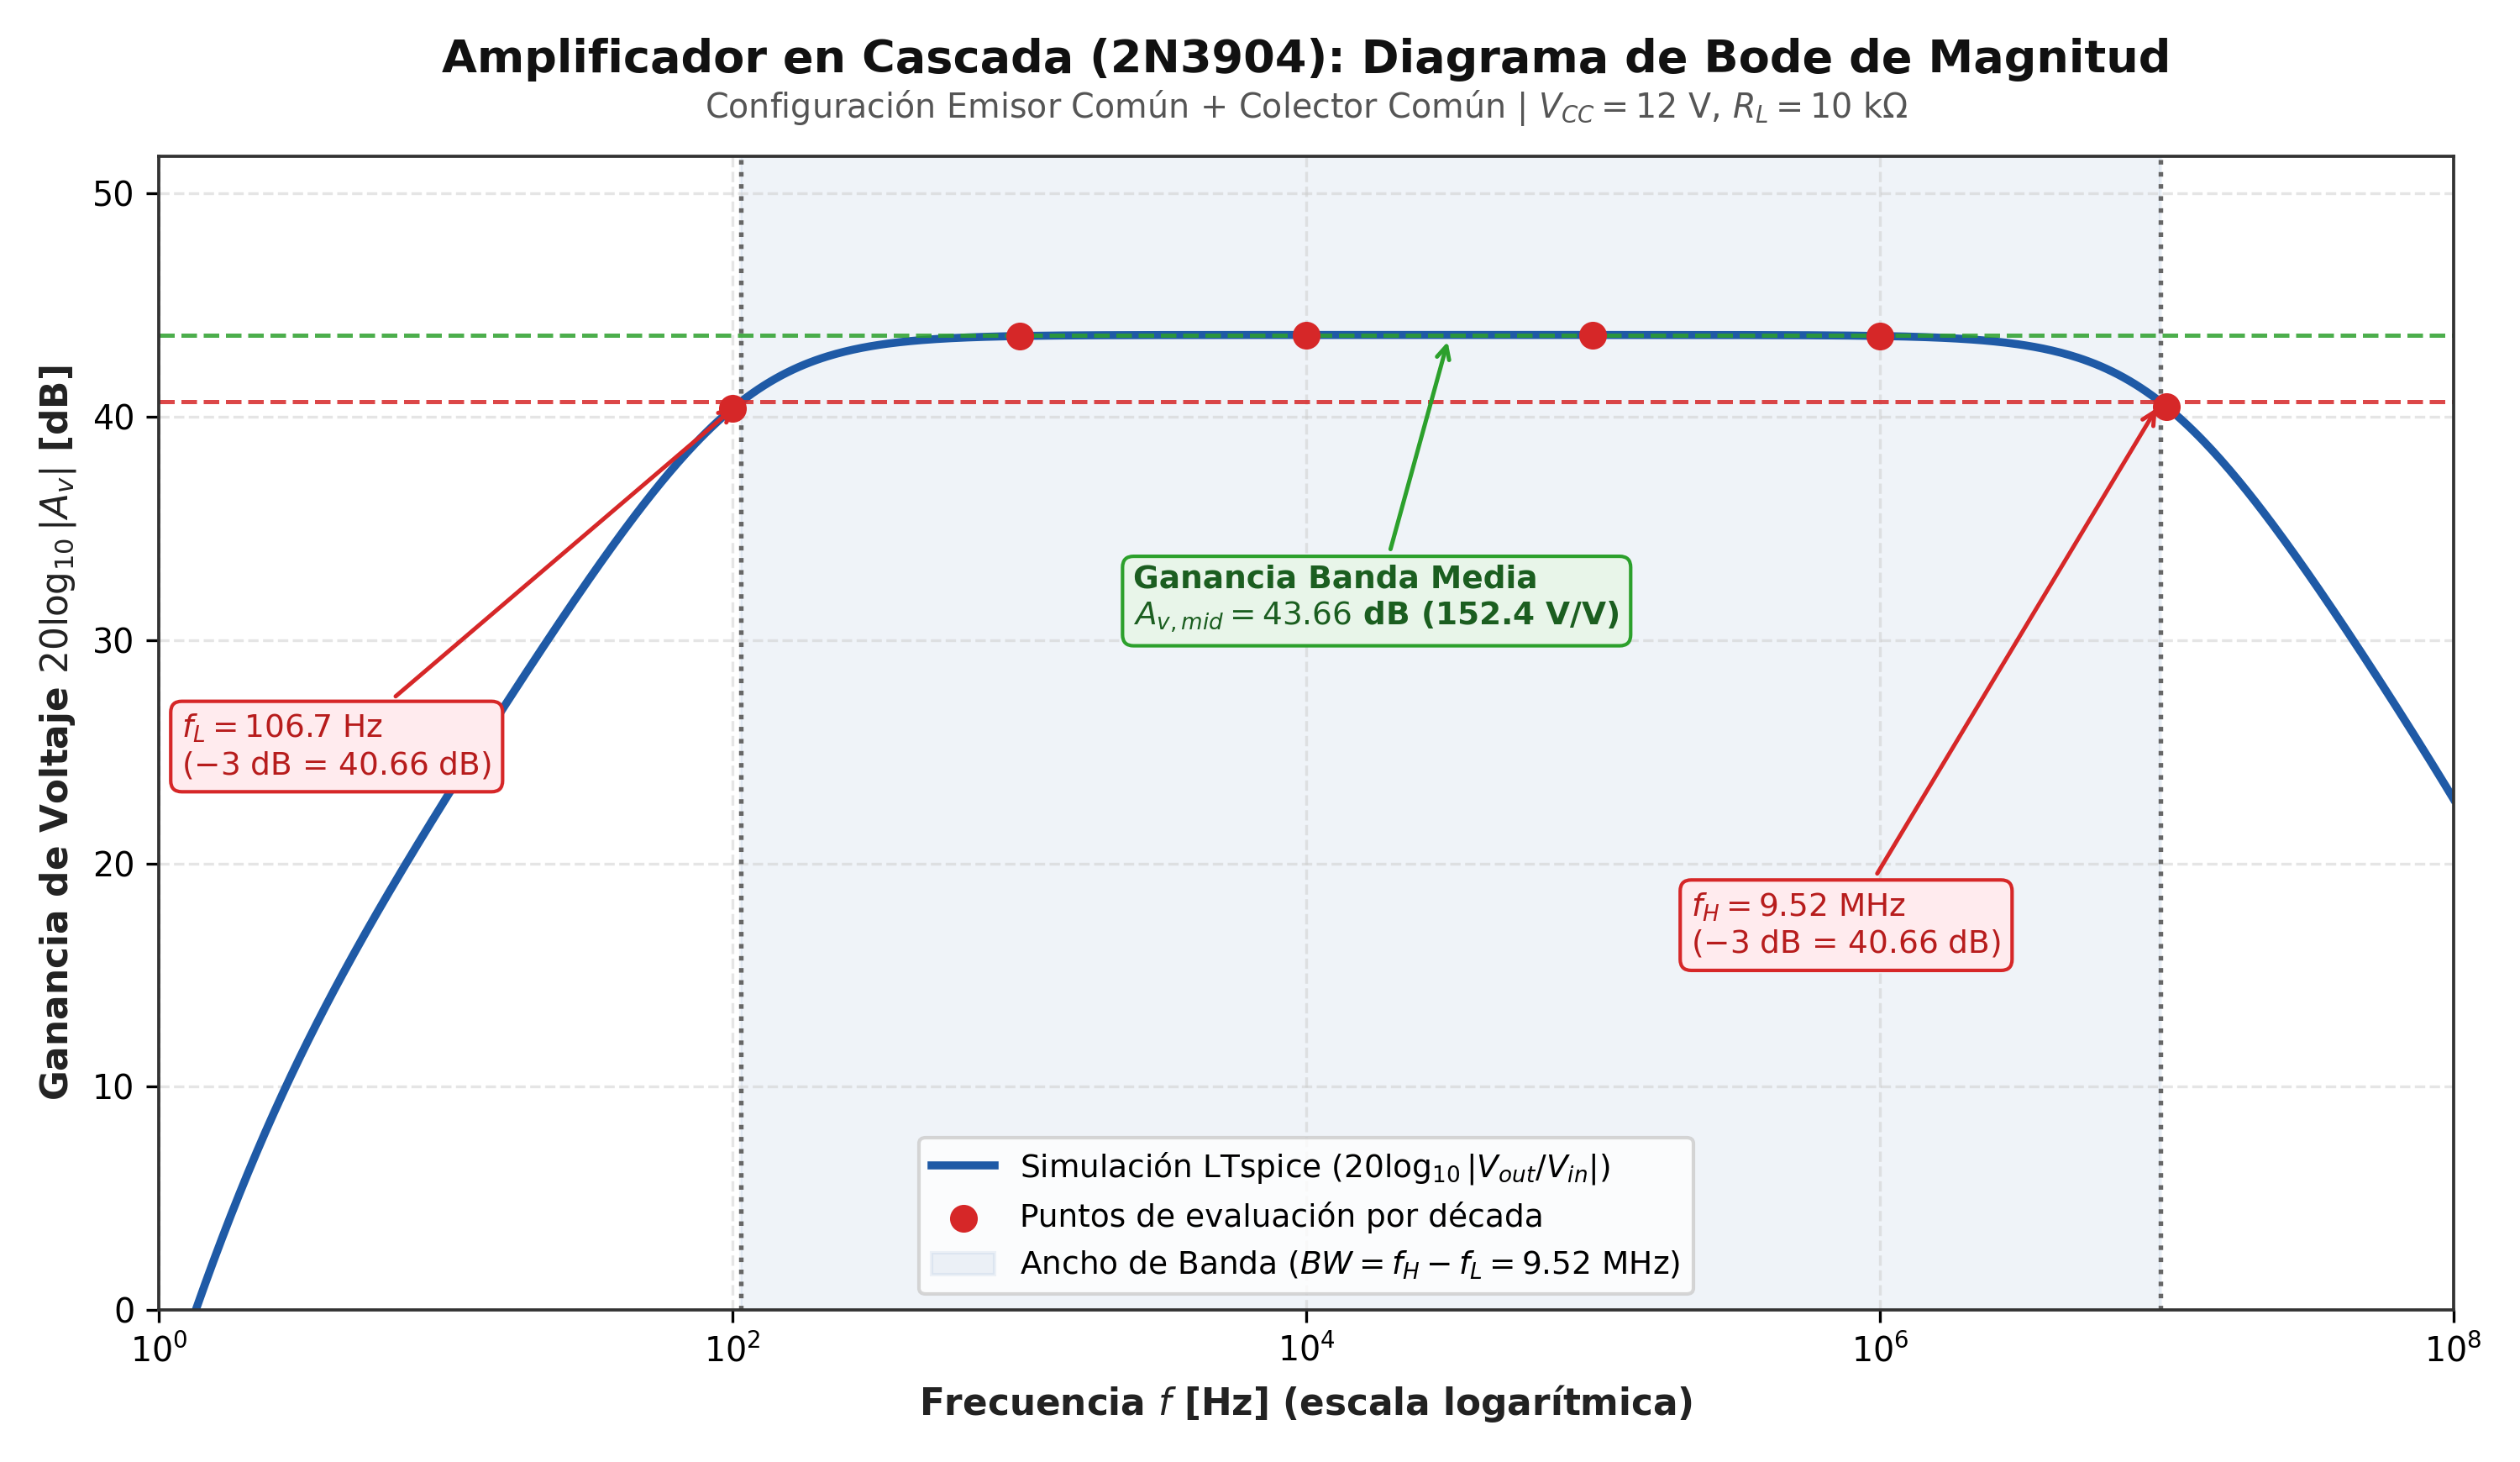
\includegraphics[width=0.84\linewidth]{AmplificadorCascadaBodeMagnitud.png}
\caption{Diagrama de Bode de magnitud del amplificador en cascada ($A_{v,\mathrm{mid}} = 43.66\text{ dB}$, $f_L = 106.7\text{ Hz}$, $f_H = 9.52\text{ MHz}$).}
\label{fig:casc_bode}
\end{figure}

% =========================================================================
% IV. MONTAJE (COMENTADO POR TRATARSE DEL PRE-INFORME DE LABORATORIO)
% Al realizar la sesión experimental, descomentar esta sección y eliminar
% la línea "\stepcounter{section}" ubicada justo antes de la Sección V.
% =========================================================================
% \section{Montaje}
%
% El montaje experimental de los circuitos dise\~nados se realizar\'a sobre protoboard empleando transistores 2N3904 previamente caracterizados, resistencias de precisi\'on y capacitores electrol\'iticos/cer\'amicos de $10\ \mu\text{F}$ y $100\ \mu\text{F}$. Los instrumentos de medici\'on corresponder\'an a la fuente de tensi\'on DC, generador de se\~nales, osciloscopio digital con sondas atenuadas ($\times 10$), sondas BNC, cables banana-caim\'an y mult\'imetro digital.
%
% % USUARIO: Insertar aquí fotografías del montaje físico y tabla de valores
% % medidos de los componentes reales y puntos de polarización DC experimentales.
% % \begin{figure}[htbp]
% % \centering
% % \includegraphics[width=0.84\linewidth]{montaje_protoboard_cascada.jpg}
% % \caption{Montaje experimental en protoboard del amplificador en cascada.}
% % \label{fig:montaje_exp}
% % \end{figure}

\stepcounter{section}
\section{An\'alisis de resultados}

Para evaluar cuantitativamente la concordancia entre los modelos anal\'iticos y los resultados obtenidos por simulaci\'on, se emplea el error relativo porcentual definido como:
\begin{equation}
\varepsilon_r = \frac{|X_{\mathrm{sim}} - X_{\mathrm{teo}}|}{|X_{\mathrm{teo}}|} \times 100\%
\label{eq:error_rel}
\end{equation}
La ecuaci\'on \eqref{eq:error_rel} permite cuantificar desviaciones atribuibles a efectos de segundo orden no incluidos en los modelos manuales simplificados. La Tabla \ref{tab:comparacion} consolida la comparaci\'on entre teor\'ia y simulaci\'on.

\begin{table}[htbp]
\centering
\caption{Comparaci\'on entre valores te\'oricos y simulados con error relativo porcentual ($\varepsilon_r$).}
\label{tab:comparacion}
\resizebox{\linewidth}{!}{%
\begin{tabular}{@{}lcccc@{}}
\toprule
Circuito / Par\'ametro & Te\'orico & Simulado & $\varepsilon_r$ (\%) & Unidad \\
\midrule
Caract. $I_{C,\mathrm{sat}}$ & $98.00$ & $99.50$ & $1.53$ & mA \\
Caract. $R_{\mathrm{frontera}}$ & $4.69$ & $3.60$ & $23.24$ & k$\Omega$ \\
Caract. $V_{CE}$ ($10\text{ k}\Omega$) & $5.40$ & $5.50$ & $1.85$ & V \\
Caract. $V_{CE}$ ($100\text{ k}\Omega$) & $9.54$ & $9.50$ & $0.42$ & V \\
\midrule
EC$^{\mathrm{a}}$ $|A_v|$ / $Z_{\mathrm{in}}$ & -- & -- & -- & -- \\
\midrule
ECD $|A_v|$ & $5.08$ & $3.90$ & $23.23$ & V/V \\
ECD $Z_{\mathrm{in}}$ & $5.62$ & $10.00$ & $77.94$ & k$\Omega$ \\
ECD $Z_{\mathrm{out}}$ & $3.13$ & $2.46$ & $21.41$ & k$\Omega$ \\
\midrule
CC $A_v$ & $0.994$ & $0.980$ & $1.41$ & V/V \\
\midrule
Cascada $|A_v|$ (tran.) & $151.87$ & $152.78$ & $0.60$ & V/V \\
Cascada $|A_v|$ (Bode) & $151.87$ & $152.40$ & $0.35$ & V/V \\
Cascada $Z_{\mathrm{in}}$ & $2.320$ & $2.373$ & $2.28$ & k$\Omega$ \\
Cascada $f_L$ & $104.9$ & $106.7$ & $1.72$ & Hz \\
Cascada $V_{\mathrm{out,max}}$ & $+4.11$ & $+4.12$ & $0.24$ & V \\
Cascada $V_{\mathrm{out,min}}$ & $-4.63$ & $-4.66$ & $0.65$ & V \\
\bottomrule
\multicolumn{5}{l}{\footnotesize $^{\mathrm{a}}$Completar al integrar la etapa EC individual y la columna experimental.}
\end{tabular}%
}
\end{table}

% USUARIO: Tras realizar el laboratorio, descomentar este párrafo para añadir
% el análisis comparativo frente a los datos experimentales de los amplificadores.
% \subsection*{Comparaci\'on con resultados experimentales}
% En la validaci\'on f\'isica se calcular\'an los errores relativos porcentuales
% entre los valores medidos en osciloscopio/mult\'imetro y las predicciones
% te\'oricas y simuladas, considerando tolerancias de resistores ($\pm 5\%$),
% capacitancia par\'asita de las sondas y dispersi\'on de $\beta$.

\subsection{An\'alisis de la caracterizaci\'on del 2N3904 y validez del modelo}

Al contrastar los c\'alculos de la Tabla \ref{tab:caract_teo} con las Figs. \ref{fig:caract_vce}--\ref{fig:caract_beta}, se observa excelente acuerdo en $V_{CE}$ dentro de la regi\'on activa ($\varepsilon_r = 1.85\%$ en $10\text{ k}\Omega$ y $0.42\%$ en $100\text{ k}\Omega$) y en $I_{C,\mathrm{sat}}$ ($\varepsilon_r = 1.53\%$). Sin embargo, la resistencia de frontera difiere en un $23.24\%$ ($4.69\text{ k}\Omega$ te\'orico frente a $3.6\text{ k}\Omega$ en SPICE) y en saturaci\'on $V_{CE,\mathrm{sat}}$ cae por debajo de los $0.20\text{ V}$ asumidos. Estas diferencias surgen porque el c\'alculo manual asume un modelo lineal por tramos con $V_{BE} = 0.7\text{ V}$ fijo y $\beta = 200$ constante, mientras que LTspice emplea el modelo no lineal de Gummel--Poon \cite{sedra2020}: a corrientes cercanas a $100\text{ mA}$, $V_{BE}$ supera $0.8\text{ V}$ por la relaci\'on exponencial de la uni\'on y la ganancia efectiva de corriente desciende por efectos de alta inyecci\'on ($I_{KF}$), desplazando la frontera hacia una menor resistencia de base. Adicionalmente, en regi\'on activa el modelo SPICE incorpora el efecto Early (modulaci\'on del ancho de base), lo cual explica por qu\'e $\beta$ crece de $171.33$ a $228.47$ conforme aumenta $V_{CE}$ en la Fig. \ref{fig:caract_beta}.

Conceptualmente, la gr\'afica de $I_C/I_B$ en funci\'on de $V_{CE}$ (Fig. \ref{fig:caract_beta}) revela dos reg\'imenes bien diferenciados: cuando $V_{CE} \lesssim 0.4\text{ V}$, ambas uniones quedan polarizadas en directa y la relaci\'on $I_C/I_B$ se desploma hacia un $\beta_{\mathrm{forzado}} \ll h_{FE}$ debido a que la corriente de colector est\'a limitada por el circuito externo; en contraste, para $V_{CE} > 0.4\text{ V}$, el transistor entra en regi\'on activa directa y la ganancia alcanza su valor nominal de amplificaci\'on ($h_{FE}$). Esta informaci\'on resulta indispensable para el resto de la pr\'actica por dos razones: primero, establece el margen m\'inimo de $V_{CE}$ necesario para evitar recorte por saturaci\'on; segundo, permite extraer la ganancia real de los ejemplares disponibles en laboratorio ($\beta_{\mathrm{prom1}} = 212.58$ y $\beta_{\mathrm{prom2}} = 246.13$, con desviaciones del $6.29\%$ y $23.07\%$ respecto al valor nominal de $200$) e integrarla en el modelo \texttt{2N3904\_LAB}, reduciendo la incertidumbre en el dise\~no de los puntos de polarizaci\'on y las impedancias de los amplificadores.

\subsection{Evaluaci\'on de los amplificadores y condiciones de polarizaci\'on}

En el amplificador en cascada se evidencia la m\'as alta precisi\'on entre teor\'ia y simulaci\'on: la ganancia de peque\~na se\~nal difiere solo en $0.60\%$ en el dominio del tiempo ($152.78\text{ V/V}$ frente a $151.87\text{ V/V}$) y $0.35\%$ en el diagrama de Bode ($152.40\text{ V/V}$), la impedancia de entrada en $2.28\%$ ($2.373\text{ k}\Omega$ frente a $2.320\text{ k}\Omega$), la frecuencia de corte inferior dominante en $1.72\%$ ($106.7\text{ Hz}$ frente a $104.9\text{ Hz}$) y los l\'imites de recorte en apenas $0.24\%$ ($+4.12\text{ V}$) y $0.65\%$ ($-4.66\text{ V}$). Esto valida f\'isicamente que la excursi\'on positiva est\'a acotada por el corte de $Q_1$ y la negativa por el corte de $Q_2$, as\'i como la pertinencia de fijar $V_{\mathrm{in}} = 10\text{ mV}_{pp}$ para garantizar operaci\'on lineal sin distorsi\'on arm\'onica apreciable.

En el colector com\'un, la ganancia simulada de $0.980\text{ V/V}$ presenta un error m\'inimo del $1.41\%$ respecto a $0.994\text{ V/V}$, confirmando el seguimiento de fase ($\Delta\phi \approx 0^\circ$) y el amplio margen en alta frecuencia ($f_H > 100\text{ MHz}$). En cuanto al emisor com\'un degenerado, las formas de onda de las Figs. \ref{fig:ecd_tran}--\ref{fig:ecd_clip} confirman cualitativamente todos los rasgos esperados de la topolog\'ia (inversi\'on de $180^\circ$, ganancia moderada estable, banda pasante de $10\text{ MHz}$ y recorte casi sim\'etrico en $+5.2\text{ V}/-5.0\text{ V}$); no obstante, la Tabla \ref{tab:comparacion} expone errores relativos elevados ($23.23\%$ en $|A_v|$, $77.94\%$ en $Z_{\mathrm{in}}$ y $21.41\%$ en $Z_{\mathrm{out}}$) junto con una frecuencia de excitaci\'on de $1\text{ kHz}$ en lugar de $10\text{ kHz}$. Esto indica que las gr\'aficas exportadas del emisor degenerado corresponden a una parametrizaci\'on preliminar distinta a los valores finales del esquem\'atico de la Fig. \ref{fig:ecd_esq}, por lo que deber\'an regenerarse con dicho esquem\'atico antes de la comparaci\'on experimental definitiva.

A partir de los dise\~nos realizados se deduce que, para que una polarizaci\'on garantice una buena amplificaci\'on, deben cumplirse cuatro condiciones fundamentales \cite{sedra2020,horowitz2015}: (i) asegurar la operaci\'on firme en la regi\'on activa directa lejos de corte y saturaci\'on; (ii) centrar el punto $Q$ respecto a la recta de carga AC para maximizar la excursi\'on sim\'etrica de salida sin recorte (como se verific\'o en $V_{CE1} = 5.783\text{ V}$ y $V_{CE2} = 5.847\text{ V}$ con $V_{CC} = 12\text{ V}$); (iii) estabilizar el punto $Q$ frente a la dispersi\'on de $\beta$ y cambios de temperatura empleando divisor de tensi\'on r\'igido y resistencia de emisor $R_E$; y (iv) respetar las especificaciones t\'ermicas y de ruptura del 2N3904 ($P_D \le 625\text{ mW}$, $I_C \le 200\text{ mA}$ y $V_{CEO} \le 40\text{ V}$ \cite{onsemi2021}), escogiendo capacitores de acoplo y desacoplo adecuados a la banda de operaci\'on.

\subsection{Comparaci\'on BJT frente a MOSFET y evaluaci\'on de configuraciones}

Respecto a las diferencias entre amplificadores con BJT y con MOSFET, el BJT es un dispositivo controlado por corriente ($I_B$) cuya resistencia de entrada $r_\pi$ es finita y moderada (del orden de $2\text{--}3\text{ k}\Omega$ en la etapa EC), mientras que el MOSFET es controlado por tensi\'on ($V_{GS}$) y presenta una impedancia de entrada virtualmente infinita en DC y bajas frecuencias \cite{sedra2020}. En contrapartida, para una misma corriente de polarizaci\'on, el BJT proporciona una transconductancia significativamente superior ($g_m = I_C/V_T$ frente a $g_m = 2I_D/V_{OV}$ en el MOSFET), logrando mayores ganancias de voltaje por etapa y menor ruido $1/f$ a bajas frecuencias; sin embargo, esta elevada transconductancia impone un rango lineal de peque\~na se\~nal mucho m\'as estrecho ($|v_{be}| \ll V_T \approx 25.85\text{ mV}$ frente a $|v_{gs}| \ll V_{OV}$) y mayor sensibilidad a la temperatura por el coeficiente negativo de $V_{BE}$ \cite{sedra2020,horowitz2015}.

Finalmente, la experiencia de dise\~no permite sintetizar las ventajas, desventajas y escenarios de aplicaci\'on de las cuatro configuraciones trabajadas:
\begin{itemize}
\item \textbf{Emisor com\'un (EC):} ofrece la mayor ganancia de voltaje (con inversi\'on de $180^\circ$), pero presenta baja $Z_{\mathrm{in}}$, sensibilidad de la ganancia a $r_e$ y la temperatura, y un rango lineal muy estrecho ($\le 10\text{ mV}_{pp}$). Resulta \'optimo como etapa inicial de amplificaci\'on para se\~nales muy d\'ebiles en receptores y preamplificadores.
\item \textbf{Emisor com\'un degenerado (ECD):} al incorporar $R_E$ sin desacoplar, incrementa $Z_{\mathrm{in}}$, extiende notablemente el margen lineal de peque\~na se\~nal y fija una ganancia altamente estable ($A_v \approx -R_{C,\mathrm{eff}}/R_E$), a costa de reducir sustancialmente la ganancia total. Es id\'oneo en etapas de instrumentaci\'on y audio donde prima la baja distorsi\'on.
\item \textbf{Colector com\'un (CC):} no amplifica tensi\'on ($A_v \approx 0.98\text{--}0.99\text{ V/V}$, sin inversi\'on), pero provee ganancia de corriente, alta impedancia de entrada ($26.41\text{ k}\Omega$), muy baja impedancia de salida ($13.87\ \Omega$) y enorme ancho de banda ($> 100\text{ MHz}$). Se emplea como b\'ufer acoplador de impedancias y etapa de salida para excitar cargas de baja resistencia.
\item \textbf{Cascada (EC + CC):} combina las virtudes de ambas etapas, logrando alta ganancia global ($152.78\text{ V/V}$), aislamiento de la carga $R_L$ respecto al colector de $Q_1$, baja $Z_{\mathrm{out}}$ ($25.26\ \Omega$) y un ancho de banda de $9.52\text{ MHz}$, con la contrapartida de mayor consumo de potencia, m\'as componentes y conservaci\'on de la baja $Z_{\mathrm{in}}$ de la etapa EC. Es ampliamente utilizada en sistemas multietapa de acondicionamiento de sensores, audio y telecomunicaciones \cite{razavi2012,horowitz2015}.
\end{itemize}

\section{Conclusiones}

\begin{enumerate}
\item La caracterizaci\'on del BJT 2N3904 demostr\'o que el modelo te\'orico lineal predice con alta precisi\'on el voltaje $V_{CE}$ en regi\'on activa ($\varepsilon_r \le 1.85\%$) y la corriente de saturaci\'on ($98.0\text{ mA}$ te\'orico frente a $99.5\text{ mA}$ simulado, $\varepsilon_r = 1.53\%$), mientras que las desviaciones en la frontera de saturaci\'on ($4.69\text{ k}\Omega$ frente a $3.6\text{ k}\Omega$, $\varepsilon_r = 23.24\%$) y en la pendiente de $\beta(V_{CE})$ evidencian la influencia del efecto Early y la alta inyecci\'on presentes en el modelo SPICE. Asimismo, la caracterizaci\'on previa de los ejemplares f\'isicos ($\beta_{\mathrm{prom1}} = 212.58$ y $\beta_{\mathrm{prom2}} = 246.13$) confirm\'o la dispersi\'on entre dispositivos y permiti\'o calibrar fielmente el modelo de simulaci\'on.
\item En el amplificador colector com\'un, el modelo anal\'itico ($A_v = 0.994\text{ V/V}$, $Z_{\mathrm{in}} = 26.41\text{ k}\Omega$, $Z_{\mathrm{out}} = 13.87\ \Omega$) concuerda estrechamente con la simulaci\'on ($A_v = 0.980\text{ V/V}$, $\varepsilon_r = 1.41\%$, desfase $0^\circ$), verificando su desempe\~no como etapa acopladora de impedancias con amplio ancho de banda.
\item El amplificador en cascada (EC + CC) valid\'o la sinergia entre alta ganancia y acoplamiento de salida, obteniendo concordancia sobresaliente entre teor\'ia y simulaci\'on en ganancia de banda media ($151.87\text{ V/V}$ frente a $152.78\text{ V/V}$, $\varepsilon_r = 0.60\%$), impedancia de entrada ($2.320\text{ k}\Omega$ frente a $2.373\text{ k}\Omega$, $\varepsilon_r = 2.28\%$), frecuencia de corte inferior ($104.9\text{ Hz}$ frente a $106.7\text{ Hz}$, $\varepsilon_r = 1.72\%$) y l\'imites de recorte ($+4.11\text{ V}/-4.63\text{ V}$ frente a $+4.12\text{ V}/-4.66\text{ V}$, $\varepsilon_r \le 0.65\%$), confirmando que el l\'imite lineal de entrada est\'a regido por $Q_1$ en $10\text{ mV}_{pp}$.
\item En la etapa de emisor com\'un degenerado, la realimentaci\'on local en emisor ampli\'o el rango lineal y estabiliz\'o la respuesta en frecuencia ($BW \approx 10\text{ MHz}$); sin embargo, las diferencias cuantitativas detectadas entre el esquem\'atico dise\~nado ($|A_v| = 5.08\text{ V/V}$, $Z_{\mathrm{in}} = 5.62\text{ k}\Omega$) y las gr\'aficas preliminares ($|A_v| = 3.90\text{ V/V}$, $Z_{\mathrm{in}} = 10.00\text{ k}\Omega$) indican la necesidad de reexportar dicha simulaci\'on con los valores definitivos antes de contrastarla con las mediciones de laboratorio.
% USUARIO: Descomentar al completar la parte experimental y el EC del compañero.
% \item La etapa individual de emisor com\'un y las mediciones experimentales
% de laboratorio consolidar\'an la validaci\'on f\'isica de las cuatro topolog\'ias.
\end{enumerate}

\begin{thebibliography}{9}

\bibitem{sedra2020}
A. S. Sedra, K. C. Smith, T. C. Carusone, and V. Gaudet, \emph{Microelectronic Circuits}, 8th ed. New York, NY, USA: Oxford University Press, 2020.

\bibitem{onsemi2021}
onsemi, \emph{2N3903, 2N3904 General Purpose Transistors NPN Silicon}, Datasheet 2N3903/D, Rev. 9, Aug. 2021.

\bibitem{webster2010}
J. G. Webster, Ed., \emph{Medical Instrumentation: Application and Design}, 4th ed. Hoboken, NJ, USA: John Wiley \& Sons, 2010.

\bibitem{razavi2012}
B. Razavi, \emph{RF Microelectronics}, 2nd ed. Upper Saddle River, NJ, USA: Pearson Education, 2012.

\bibitem{fortescue2011}
P. Fortescue, G. Swinerd, and J. Stark, Eds., \emph{Spacecraft Systems Engineering}, 4th ed. Hoboken, NJ, USA: John Wiley \& Sons, 2011.

\bibitem{horowitz2015}
P. Horowitz and W. Hill, \emph{The Art of Electronics}, 3rd ed. Cambridge, U.K.: Cambridge University Press, 2015.

\end{thebibliography}

\end{document}